\documentclass[12pt]{article}
% ---------- fonts: Times text and math, Helvetica sans, Courier mono ----------
\usepackage[utf8]{inputenc}
\usepackage[T1]{fontenc}
\usepackage{mathptmx}
\usepackage[scaled=0.92]{helvet}
\usepackage{courier}
\usepackage{textcomp}
\usepackage[expansion=false]{microtype}

% ---------- page layout ----------
\usepackage[a4paper,margin=1in,headheight=14pt]{geometry}
\usepackage{setspace}
\onehalfspacing
\setlength{\parskip}{0pt}
\setlength{\parindent}{1.5em}
\setlength{\emergencystretch}{2em}
\usepackage{fancyhdr}
\pagestyle{fancy}
\fancyhf{}
\fancyhead[R]{\small\itshape Decision-Focused Volatility Timing}
\fancyfoot[C]{\small\thepage}
\renewcommand{\headrulewidth}{0pt}
\fancypagestyle{plain}{\fancyhf{}\fancyfoot[C]{\small\thepage}\renewcommand{\headrulewidth}{0pt}}

% ---------- headings ----------
\usepackage{titlesec}
\titleformat{\section}{\normalfont\large\bfseries}{\thesection.}{0.6em}{}
\titleformat{\subsection}{\normalfont\normalsize\bfseries}{\thesubsection}{0.6em}{}
\titleformat{\subsubsection}{\normalfont\normalsize\bfseries\itshape}{}{0em}{}
\titleformat{\paragraph}[runin]{\normalfont\normalsize\itshape}{}{0em}{}
\titlespacing*{\section}{0pt}{2.2ex plus 1ex minus .2ex}{1.2ex plus .2ex}
\titlespacing*{\subsection}{0pt}{1.8ex plus 1ex minus .2ex}{0.8ex plus .2ex}
\titlespacing*{\subsubsection}{0pt}{1.5ex plus .5ex minus .2ex}{0.5ex}
\titlespacing*{\paragraph}{0pt}{1.0ex plus .5ex minus .2ex}{0.6em}

% ---------- maths, tables, figures ----------
\usepackage{amsmath,amssymb}
\usepackage{booktabs,tabularx,multirow,array}
\usepackage{graphicx}
\usepackage{adjustbox}
\usepackage{caption}
\captionsetup{font={small,singlespacing}, labelfont=bf, labelsep=period, justification=justified, singlelinecheck=true}
\captionsetup[table]{position=top, skip=6pt}
\captionsetup[figure]{skip=6pt}
\usepackage{subcaption}
\usepackage{float}
\usepackage[section]{placeins}
\renewcommand{\arraystretch}{1.15}
\setlength{\abovecaptionskip}{6pt}
\setlength{\textfloatsep}{14pt plus 2pt minus 4pt}

% ---------- lists, colour, diagrams, links ----------
\usepackage{enumitem}
\setlist{itemsep=1pt, topsep=3pt, parsep=0pt}
\usepackage{xcolor}
\definecolor{linkblue}{HTML}{1F3A80}
\usepackage{tikz}
\usetikzlibrary{shapes.geometric,shapes.misc,arrows.meta,positioning,calc}
\usepackage[colorlinks=true, linkcolor=linkblue, citecolor=linkblue, urlcolor=linkblue]{hyperref}
\urlstyle{same}

% ---------- unicode in the source ----------
\usepackage{newunicodechar}
\newunicodechar{−}{\ensuremath{-}}
\newunicodechar{²}{\textsuperscript{2}}
\newunicodechar{γ}{\ensuremath{\gamma}}
\newunicodechar{σ}{\ensuremath{\sigma}}
\newunicodechar{μ}{\ensuremath{\mu}}
\newunicodechar{κ}{\ensuremath{\kappa}}
\newunicodechar{≥}{\ensuremath{\geq}}
\newunicodechar{≤}{\ensuremath{\leq}}
\newunicodechar{≈}{\ensuremath{\approx}}
\newunicodechar{×}{\ensuremath{\times}}
\newunicodechar{±}{\ensuremath{\pm}}
\newunicodechar{√}{\ensuremath{\surd}}

% ---------- project macros ----------
\newcommand{\VIX}{VIX\textsuperscript{2}}
% questions: left-aligned, "Question." then the examiner's text, then "Answer." runs into our reply
\newenvironment{question}{\par\smallskip\noindent\textbf{Question.}\ \itshape}{\par\smallskip\noindent\upshape\textbf{Answer.}\ \ignorespacesafterend}
\newcommand{\tablenote}[1]{\par\smallskip\parbox{\linewidth}{\footnotesize\singlespacing #1}}

% appendices: "Appendix A. Title", on their own pages
\newcommand{\startappendices}{%
  \clearpage
  \appendix
  \titleformat{\section}{\normalfont\large\bfseries}{Appendix \thesection.}{0.6em}{}
  \begin{center}\normalfont\Large\bfseries Appendices\end{center}
  \addcontentsline{toc}{section}{Appendices}
  \vspace{1ex}}


\begin{document}
\thispagestyle{plain}
\begin{center}
{\LARGE\bfseries Decision-Focused Volatility Timing\par}
\vspace{0.8em}
{\large Does a better volatility forecast, or one trained for the trading decision,\\ make a volatility-managed portfolio work out of sample?\par}
\vspace{1.4em}
{\normalsize Hanyang University\par}
\vspace{1.2em}
{\normalsize Team 6\par}
\vspace{1.5em}
{\normalsize November 2026\par}
\vspace{1.2em}
{\footnotesize Term project, Introduction to Financial Engineering, Hanyang University.\par}
\end{center}
\vspace{0.8em}
\begin{center}{\bfseries Abstract}\end{center}
\vspace{-0.6em}
\begin{singlespace}\small
\noindent Volatility-managed portfolios hold less of an asset when its variance is expected to be high (Moreira and Muir, 2017). We rebuild the strategy in a pseudo-out-of-sample test on the US equity market from January 1998 to December 2025 (336 months), net of 10 bp trading costs, and study two extensions. First, we run the strategy with a richer variance forecast than backward-looking realised variance: the GARCH-LSTM of Zhao et al.\ (2024), a GJR-GARCH whose daily variance is rescaled by a small LSTM network, compared with GARCH(1,1), GJR-GARCH and two controls (last month's realised variance and \VIX). Second, we train the GARCH-LSTM on the investor's utility of the timed portfolio, with the trading rule, its leverage cap and costs inside the loss, rather than on forecast accuracy (decision-focused learning, Elmachtoub and Grigas, 2022). We find that timing is a risk tool, not a return engine: the four RV/GARCH-based portfolios roughly halve the worst month-end drawdown of the market ($-$50\% to between $-$21\% and $-$29\%) and lower volatility by about 30\%, but the Sharpe gain ($+$0.08 to $+$0.10) is not statistically significant and comes from before 2016. A better forecast does not give a better portfolio: the accuracy ranking of the five forecasts is close to the reverse of their Sharpe ranking. The most accurate forecast, \VIX{} (QLIKE 0.275), gives the lowest Sharpe ratio (0.545) and the least accurate, last month's realised variance (QLIKE 0.454), the highest (0.612), because variance is predictable one month ahead while returns are not, and a sharper variance forecast cuts exposure harder in the high-return recovery months. Decision-focused training does not help either: against the accuracy-trained network it lowers its own out-of-sample objective on average ($-$0.45\% a year) and the Sharpe ratio on 4 of 6 Fama--French factors, makes its forecasts 1.3 to 5.8 times worse, and no difference survives a multiple-testing adjustment.
\end{singlespace}
\vspace{0.8em}
\begin{singlespace}\small
\noindent\textit{JEL classification:} G11, G12, G17, C22, C45, C53.\\[2pt]
\noindent\textit{Keywords:} volatility-managed portfolios, volatility timing, GARCH, GARCH-LSTM, decision-focused learning, forecast evaluation, out-of-sample testing.
\end{singlespace}
\clearpage

%======================================================================
\section{Overview}
\subsection{Motivation}
Moreira and Muir (2017) show that scaling exposure to the market, or to an equity factor, by the inverse of last month's realised variance raises its Sharpe ratio; Barroso and Santa-Clara (2015) find the same for momentum. Cederburg et al.\ (2020) then show that, once the strategy is built in real time with only the information available at each decision, most of these gains shrink or vanish. Our angle is the forecast that drives the rule. The original strategy uses a naive, backward-looking forecast (last month's realised variance). We examine two possible extensions in this setting:
\begin{enumerate}[label=(\roman*)]
\item a better forecasting model, the hybrid GARCH-LSTM of Zhao et al.\ (2024), which is more accurate than classical GARCH models in their tests; and
\item a forecast trained for the decision it feeds. Volatility models are normally fitted to maximise forecast accuracy (a quasi-likelihood). Decision-focused learning (Elmachtoub and Grigas, 2022) instead trains the forecast on the quality of the decision, here the investor's utility of the timed portfolio after costs.
\end{enumerate}
We organise the project around three questions:
\begin{description}[labelwidth=2em,leftmargin=3em]
\item[Q1] Does volatility timing beat buy and hold of the market in real time?
\item[Q2] Does a better (more accurate) volatility forecast give a better portfolio?
\item[Q3] Does training the forecast for the trading decision, instead of for accuracy, fix it?
\end{description}

\subsection{Overall design of the investment strategy}
Figure~\ref{fig:process} summarises the strategy. Each month it (1) collects data dated before the decision, (2) forecasts next month's market variance with one of five forecasts, (3) turns the forecast into a market exposure with a single fixed rule, $w_t=\min(c_t/\hat v_t,\,1.5)$, (4) holds that exposure for one month in a portfolio of the market and cash, paying 10 bp on every unit of exposure traded, and (5) is evaluated against buy and hold with block-bootstrap and HAC tests. The rule, the cap, the costs, the benchmark and the tests are the same for every portfolio; the portfolios differ in the forecast and, for Q3, in the objective the forecast is trained on. The forecasts come from two estimation procedures (Section~\ref{sec:design}), and we check that this difference does not drive the results.

\subsection{Key findings}
\begin{enumerate}
\item \textbf{Q1: Timing is a risk tool, not a return engine.} The four RV/GARCH-based portfolios roughly halve the worst month-end drawdown of the market ($-$50.3\% to between $-$21.3\% and $-$29.4\%; $-$32\% to $-$42\% even after rescaling to the market's volatility), lost less than buy and hold in five of six crises, cut volatility from 15.9\% to about 11\% a year, and raise the Sortino ratio and the certainty-equivalent return. The only statistically significant improvement is a steadier portfolio risk (vol of vol at equal volatility, GARCH(1,1), GJR-GARCH and GARCH-LSTM, $p=0.005$ to $0.033$ before adjustment). The Sharpe gain ($+$0.08 to $+$0.10) is not significant and comes from 1998--2015. Because the timed portfolios hold less risk, they end with less wealth than the market: \$1 grows to \$9.5--\$9.9 against \$12.3.
\item \textbf{Q2: A better forecast does not give a better portfolio.} Ranked from most to least accurate (QLIKE), the forecasts are \VIX{} (0.275), GARCH-LSTM (0.280), GJR-GARCH (0.284), GARCH(1,1) (0.297) and last month's realised variance (0.454); ranked by Sharpe ratio, the order is almost reversed: RV 0.612, GARCH 0.608, GJR and GARCH-LSTM 0.597, \VIX{} 0.545 (rank correlation $-$0.9). Splitting the Sharpe ratio into variance timing and mean timing shows that variance timing works for every forecast (1.21 to 1.29) while mean timing falls from 1.01 to 0.90 as forecasts become more informative.

\textit{Why.} Variance is predictable one month ahead (out-of-sample $R^2$ of 47\% to 57\%), returns are not (every standard predictor does worse than the historical average). The rule therefore times variance with a constant expected return and holds little of the market in the ``recovery'' months, when volatility is high but falling and returns are highest.
\item \textbf{Q3: Training for the decision does not help.} Against the accuracy-trained GARCH-LSTM, the decision-trained network has a lower realised objective on average ($-$0.45\% a year; higher on only 2 of 6 factors) and a lower Sharpe ratio on 4 of 6 factors (average $-$0.02). Its forecasts are 1.3 to 5.8 times worse in QLIKE, and no difference survives the Romano--Wolf adjustment. On the market it is the weakest timed portfolio (Sharpe 0.537, worst drawdown $-$37.9\%).
\end{enumerate}

\begin{figure}[p]
\centering
\definecolor{qnavy}{HTML}{1F3A5F}
\definecolor{qteal}{HTML}{3E6D96}
\definecolor{qred}{HTML}{EEF1F5}
\definecolor{qblue}{HTML}{DCE6F2}
\definecolor{qolive}{HTML}{4A4A4A}
\definecolor{qorange}{HTML}{555555}
\begin{tikzpicture}[font=\footnotesize, node distance=6mm,
  term/.style={rounded rectangle, fill=qolive, text=white, align=center, minimum width=3.2cm, inner sep=4pt},
  dia/.style={diamond, aspect=2.1, fill=qnavy, text=white, align=center, inner sep=1pt, text width=2.9cm},
  dteal/.style={dia, fill=qteal},
  box/.style={rectangle, fill=qred, draw=qnavy!45, text=black, align=center, text width=4.0cm, inner sep=3pt, font=\scriptsize},
  para/.style={trapezium, trapezium left angle=75, trapezium right angle=105, fill=qblue, draw=qnavy!45, text=black, align=center, text width=3.4cm, inner sep=2pt, font=\scriptsize},
  arr/.style={-{Latex[length=2mm]}, qorange, thick},
  lab/.style={text=qorange, font=\scriptsize\itshape, align=left}]
\node[term] (q) {QUESTION\\ \scriptsize Does volatility timing\\ \scriptsize work in real time?};
\node[dia, below=6mm of q] (collect) {Collect data\\ \scriptsize dated before the decision};
\node[dia, below=7mm of collect] (fc) {Forecast next-month\\ market variance $\hat v_t$};
\node[dteal, below=7mm of fc] (train) {How is the\\ forecast trained?\\ (Q3)};
\node[dia, below=9mm of train] (set) {Set exposure\\ $w_t=\min(c_t/\hat v_t,\,1.5)$};
\node[dia, below=7mm of set] (hold) {Hold for one month\\ \scriptsize market + T-bills};
\node[dia, below=7mm of hold] (eval) {Evaluate against\\ buy and hold\\ \scriptsize (S\&P 500 proxy)};
\node[term, below=6mm of eval] (ans) {ANSWER\\ \scriptsize A risk tool, not a return engine};
\foreach \a/\b in {q/collect, collect/fc, fc/train, train/set, set/hold, hold/eval, eval/ans} \draw[arr] (\a) -- (\b);
% right-hand boxes
\node[box, right=8mm of collect] (b1) {Daily \& monthly returns, 1963--2025: US market (CRSP VW) and 5 Fama--French factors; VIX; 1-month T-bill};
\node[box, right=8mm of fc, yshift=5mm] (b2) {Models: GARCH(1,1); GJR-GARCH and GARCH-LSTM (5-seed ensemble), one training run};
\node[box, below=1mm of b2] (b3) {Controls: last month's RV, \VIX};
\node[para, right=8mm of train, yshift=5mm] (acc) {\textbf{Acc}: quasi-likelihood of daily returns};
\node[para, below=1.5mm of acc] (dec) {\textbf{Dec}: investor utility of the timed portfolio, with the rule inside the loss};
\node[box, right=8mm of set] (b4) {$c_t$ reset every January: capped strategy matches buy-and-hold volatility on past data};
\node[box, right=8mm of hold] (b5) {10\,bp per unit of exposure traded; leverage $\le 0.5$ at the risk-free rate};
\node[box, right=8mm of eval, yshift=5mm] (b6) {Return, volatility, Sharpe, Sortino, max drawdown, CER; sub-periods and 6 crises};
\node[box, below=1mm of b6] (b7) {Block bootstrap, Ledoit--Wolf and Romano--Wolf tests};
\draw[arr] (collect.east) -- (b1.west);
\draw[arr] (fc.east) -- ++(3mm,0) |- (b2.west);
\draw[arr] (fc.east) -- ++(3mm,0) |- (b3.west);
\draw[arr] (train.east) -- ++(3mm,0) |- (acc.west);
\draw[arr] (train.east) -- ++(3mm,0) |- (dec.west);
\draw[arr] (set.east) -- (b4.west);
\draw[arr] (hold.east) -- (b5.west);
\draw[arr] (eval.east) -- ++(3mm,0) |- (b6.west);
\draw[arr] (eval.east) -- ++(3mm,0) |- (b7.west);
\draw[arr, dashed] (dec.south) -- ++(0,-3mm) -| ($(train.south)!0.55!(set.north)$) node[lab, pos=0.25, below] {Dec: same rule, cap, costs and January $c$};
% feedback loops on the left
\draw[arr] (hold.west) -- ++(-12mm,0) |- (fc.west) node[lab, pos=0.25, right] {next month:\\ new forecast};
\draw[arr] (eval.west) -- ++(-24mm,0) |- (collect.west) node[lab, pos=0.25, left] {every January:\\ refit models\\ on past data};
\end{tikzpicture}

\caption{Process diagram of the investment strategy. Every month the strategy forecasts next month's market variance, turns the forecast into an exposure with one fixed rule, holds it for a month and is evaluated against buy and hold. The rule, the cap, the January reset of $c$, the costs, the benchmark and the tests are held fixed; the forecast (Q1, Q2) and the objective it is trained on (Q3) differ between the portfolios compared. Every input is dated before the month it is used for (expanding window, test period 1998--2025).}
\label{fig:process}
\end{figure}

%======================================================================
\section{Portfolio management framework}
\subsection{Investment universe and asset selection}
The strategy is a market-timing strategy, not a stock-picking one: each month it splits capital between a single risky asset, the US equity market, and cash. The selection question is therefore which risky asset to time and which data to forecast it with. Table~\ref{tab:data} lists the series.
\begin{itemize}
\item \textbf{Risky asset: the US market.} The CRSP value-weighted index of all US common stocks, in excess of the one-month T-bill (Ken French's Mkt-RF), daily and monthly from July 1963. It moves almost one for one with the S\&P 500, whose constituents make up most of its capitalisation. It is the asset of Moreira and Muir (2017) and Cederburg et al.\ (2020), which makes the results comparable.
\item \textbf{Five more equity factors} (SMB, HML, RMW, CMA and momentum, from the Ken French library) are used for the decision-training test (Q3) and for Appendix~\ref{app:factors}. They are long--short portfolios, hence already excess returns. All six series, including the market, are used from July 1963, from the same files, for every model.
\item \textbf{Cash.} The one-month T-bill rate (Ken French). Cash earns it, and leverage is financed at it.
\item \textbf{VIX} (CBOE, FRED series VIXCLS) is only used for the \VIX{} control forecast. CBOE back-calculated the current VIX before 2003, so those values were not observable at the time.
\item \textbf{Course CRSP stocks} (2000--2020, 6,972 stocks in February 2000 to 4,268 in December 2020) build an equal-weighted passive benchmark (Section~\ref{sec:otherbench}). \texttt{ADJ\_PRC} is split- and dividend-adjusted, so price changes are total returns; stock-months without a price are dropped (no delisting returns, Shumway, 1997).
\end{itemize}

\begin{table}[htbp]
\centering\small
\caption{Data and pre-processing.}\label{tab:data}
\begin{tabularx}{\textwidth}{@{}p{3.1cm}p{3.0cm}Xp{3.6cm}@{}}
\toprule
Series & Source & Coverage & Role\\
\midrule
US market (Mkt-RF) & Ken French, CRSP VW & 1963-07 to 2025-12, daily \& monthly & Risky asset, benchmark (Q1, Q2)\\
SMB, HML, RMW, CMA, Mom & Ken French & idem & Decision training (Q3), App.~\ref{app:factors}\\
VIX & FRED (VIXCLS) & 1990 on (back-calculated before 2003) & Control forecast \VIX\\
Risk-free rate & Ken French, 1-month T-bill & 1963 on & Cash return, financing\\
Course CRSP stocks & CRSP monthly extract & 2000-02 to 2020-12 & Equal-weighted benchmark\\
\bottomrule
\end{tabularx}
\end{table}

\paragraph{Realised variance.} The realised variance of month $t$ is the sum of its squared daily excess returns, $RV_t=\sum_{d\in t} r_d^2$, without subtracting the month's mean (Andersen and Bollerslev, 1998). Moreira and Muir (2017, eq.~2) subtract it; doing so moves the timed Sharpe ratio from 0.612 to 0.616, so the choice is immaterial. Forecast accuracy is measured against the same realised variance, rebuilt from the daily file.

\paragraph{Data vintage.} The Ken French files are rebuilt from the current (August 2026) CRSP database, so past returns are today's revised values. Every decision uses only observations dated before it, but from revised history: the backtest is a pseudo-out-of-sample test.

\subsection{Train, validation and test design}\label{sec:design}
All models are estimated on an expanding window, and every forecast for a year uses only data dated before that year. There is no shuffling and no look-ahead. Two procedures are used.
\begin{itemize}
\item \textbf{GARCH(1,1)} has three parameters and is refitted every January by quasi-maximum likelihood on all daily returns from July 1963 up to the previous December (first fit in 1970); it then forecasts the twelve months of the new year, which it has never seen. It needs no validation set.
\item \textbf{GJR-GARCH and the GARCH-LSTM} come from one training run on the same 1963 files, in the notebook \texttt{lstm\_training\_revised.ipynb}. For a test year $Y$, parameters are fitted on data before January of $Y-5$; the five calendar years $Y-5$ to $Y-1$ form a validation block, used only to choose when to stop training (and, for the decision objective of Section~\ref{sec:dec}, which checkpoint to keep). The selected model then filters all data up to each forecast date and forecasts the twelve months of $Y$. Every model is initialised afresh each year; nothing trained on a later year is reused. Parameters are not refitted on the validation years, so they are up to five years older than those of GARCH(1,1). The first test year of this run is 1975.
\end{itemize}
The scale $c$ needs at least 24 months of history, so the first positions date from the 1970s, long before the test sample. The test period is January 1998 to December 2025 (336 months), with three sub-periods (1998--2015, 2016--2025, 2021--2025) and six crisis episodes.

\FloatBarrier
\subsection{Time-series models for the variance forecast}
The rule needs $\hat v_t$, a forecast of next month's market variance made at the close of month $t-1$. We compare three models and two controls (Table~\ref{tab:forecasts}). Table~\ref{tab:notation} lists the notation used in the rest of the report: the index $d$ counts trading days and $t$ months.

\begin{table}[htbp]
\centering\small
\caption{Notation.}\label{tab:notation}
\begin{adjustbox}{max width=\linewidth}\begin{tabular}{@{}ll@{}}
\toprule
Symbol & Meaning\\
\midrule
$r_d$ & daily excess return of the market (or factor) on day $d$\\
$h_d$ & variance of $r_d$ forecast by the model with data up to day $d-1$\\
$\omega,\alpha,\beta,\delta$ & GARCH parameters ($\delta$: extra reaction to falls in GJR-GARCH)\\
$f_t$ & excess return of the market (or factor) in month $t$\\
$r^f_t$ & one-month T-bill rate in month $t$\\
$RV_t$ & realised variance of month $t$, $\sum_{d\in t} r_d^2$\\
$\hat v_t$ & forecast of $RV_t$ made at the end of month $t-1$\\
$w_t$ & exposure to the market in month $t$ (the rest in T-bills)\\
$c_t$ & scale of the rule (a target variance), reset every January\\
$z_t$ & net excess return of the portfolio in month $t$, after costs\\
$\kappa$ & trading cost, 10 bp per unit of exposure traded\\
$\gamma$ & risk aversion of the investor, $\gamma=5$\\
\bottomrule
\end{tabular}\end{adjustbox}
\end{table}

\paragraph{GARCH(1,1)} (Bollerslev, 1986). Tomorrow's variance is a weighted sum of a constant, today's squared return and today's variance:
\begin{equation}
h_d=\omega+\alpha\, r_{d-1}^2+\beta\, h_{d-1},\qquad \omega>0,\ \alpha,\beta\ge 0,\ \alpha+\beta<1.
\end{equation}
The parameters are estimated by quasi-maximum likelihood, i.e.\ by minimising $\frac1D\sum_{d=1}^{D}\bigl(\log h_d+r_d^2/h_d\bigr)$ over the $D$ training days.

\paragraph{GJR-GARCH} (Glosten et al., 1993) adds a leverage term so that variance reacts more to falls than to rises (Black, 1976):
\begin{equation}
h_d=\omega+\alpha\, r_{d-1}^2+\delta\, r_{d-1}^2\,\mathbf 1[r_{d-1}<0]+\beta\, h_{d-1},
\end{equation}
where $\mathbf 1[r_{d-1}<0]$ equals 1 after a down day and 0 otherwise. Its persistence, how slowly a shock to variance dies out, is $\phi=\alpha+\beta+\delta/2<1$ (for GARCH(1,1), $\delta=0$ and $\phi=\alpha+\beta$). The recursion is linear in the squared shocks once the parameters are fixed, so the whole variance path is computed exactly as one FFT convolution. The conditional mean is set to zero. GJR-GARCH is fitted by L-BFGS on the quasi-likelihood above, on the fitting window of Section~\ref{sec:design}.

\paragraph{Monthly forecast.} Let $T$ be the last trading day of month $t-1$ and $h_{T+1}$ the model's variance forecast for the next day. Further ahead the daily forecast reverts geometrically, at rate $\phi$, to the long-run variance $\bar h=\omega/(1-\phi)$; the monthly forecast adds the next 21 daily forecasts:
\begin{equation}\label{eq:monthly}
\hat v_t=\sum_{k=1}^{21}\Bigl[\bar h+\phi^{k-1}\bigl(h_{T+1}-\bar h\bigr)\Bigr].
\end{equation}

\paragraph{GARCH-LSTM} (Zhao et al., 2024, eq.~7). A GJR-GARCH whose daily variance is rescaled by a small LSTM network (hidden size 8) that reads the last 126 trading days (about half a year) of returns and variances. Each day the GJR formula gives a first value $g_d$, and the LSTM multiplies it by a correction factor:
\begin{equation}
h_{d+1}=g_d\times\Bigl(1+\sum_{j=1}^{8} a_j\tanh(s_{d,j})\Bigr),\qquad g_d=\omega+\alpha r_d^2+\delta r_d^2\mathbf 1[r_d<0]+\beta h_d,
\end{equation}
where $s_d$ is the LSTM's memory (its cell state, updated from $r_d$ and $h_d$) and $a_1,\dots,a_8$ are weights with $\sum_j|a_j|<1$, so the variance stays positive. The weights $a_j$ start at zero, so the network starts exactly at the GJR fit and only departs from it if the data push it. The one-day-ahead variance is carried 21 days forward with eq.~\eqref{eq:monthly} (an approximation: the network is not run forward over the month). Each year the network is initialised from that year's GJR fit and trained by Adam on random batches of 64 windows of 126 days (up to 400 steps); the validation loss is checked every 10 steps and training stops after 60 steps without improvement, keeping the best checkpoint. This is repeated for five random seeds, and the five monthly variance forecasts are averaged before the exposure is set (an ensemble), so that one lucky seed cannot drive the result.

\paragraph{Controls.} \textit{RV}: last month's realised variance, the naive ``volatility is persistent'' forecast of Moreira and Muir (2017). \textit{\VIX}: the option market's expectation of variance, the squared VIX at the previous month end converted to a monthly variance (VIX$^2$/12, with the VIX in decimals); it contains the variance risk premium.

\begin{table}[htbp]
\centering\small
\caption{The five variance forecasts and their accuracy on the US market, 1998--2025. QLIKE is the average over months of $RV_t/\hat v_t-\log(RV_t/\hat v_t)-1$ (Patton, 2011): 0 for a perfect forecast, lower is better.}\label{tab:forecasts}
\begin{tabularx}{\textwidth}{@{}llXr@{}}
\toprule
Forecast & Role & Description & QLIKE\\
\midrule
GARCH(1,1) & model & Bollerslev (1986), QML on daily returns, refitted every January & 0.297\\
GJR-GARCH & model & GARCH plus leverage term (Glosten et al., 1993), revised training run & 0.284\\
GARCH-LSTM & model & GJR-GARCH rescaled by an LSTM over 126 days (Zhao et al., 2024); ensemble of 5 seeds & 0.280\\
RV & control & Last month's realised variance (Moreira--Muir forecast) & 0.454\\
\VIX & control & Option-implied variance, from 1990 & \textbf{0.275}\\
\bottomrule
\end{tabularx}
\end{table}

Figure~\ref{fig:forecasts} plots each forecast against the realised volatility that followed. All models track the ups and downs of volatility; they differ in how fast they react and how far they overshoot. RV reacts fully to every spike and is the least accurate; GARCH(1,1) smooths it, GJR adds the leverage effect, and the GARCH-LSTM improves on its GJR base only slightly (QLIKE 0.280 against 0.284). \VIX{} lies above realised volatility most of the time because of the variance risk premium, yet it is the most accurate over the full sample, thanks to 2016--2025; GJR and the GARCH-LSTM are the most accurate in 1998--2015 (Appendix~\ref{app:checks}).

\begin{figure}[htbp]
\centering
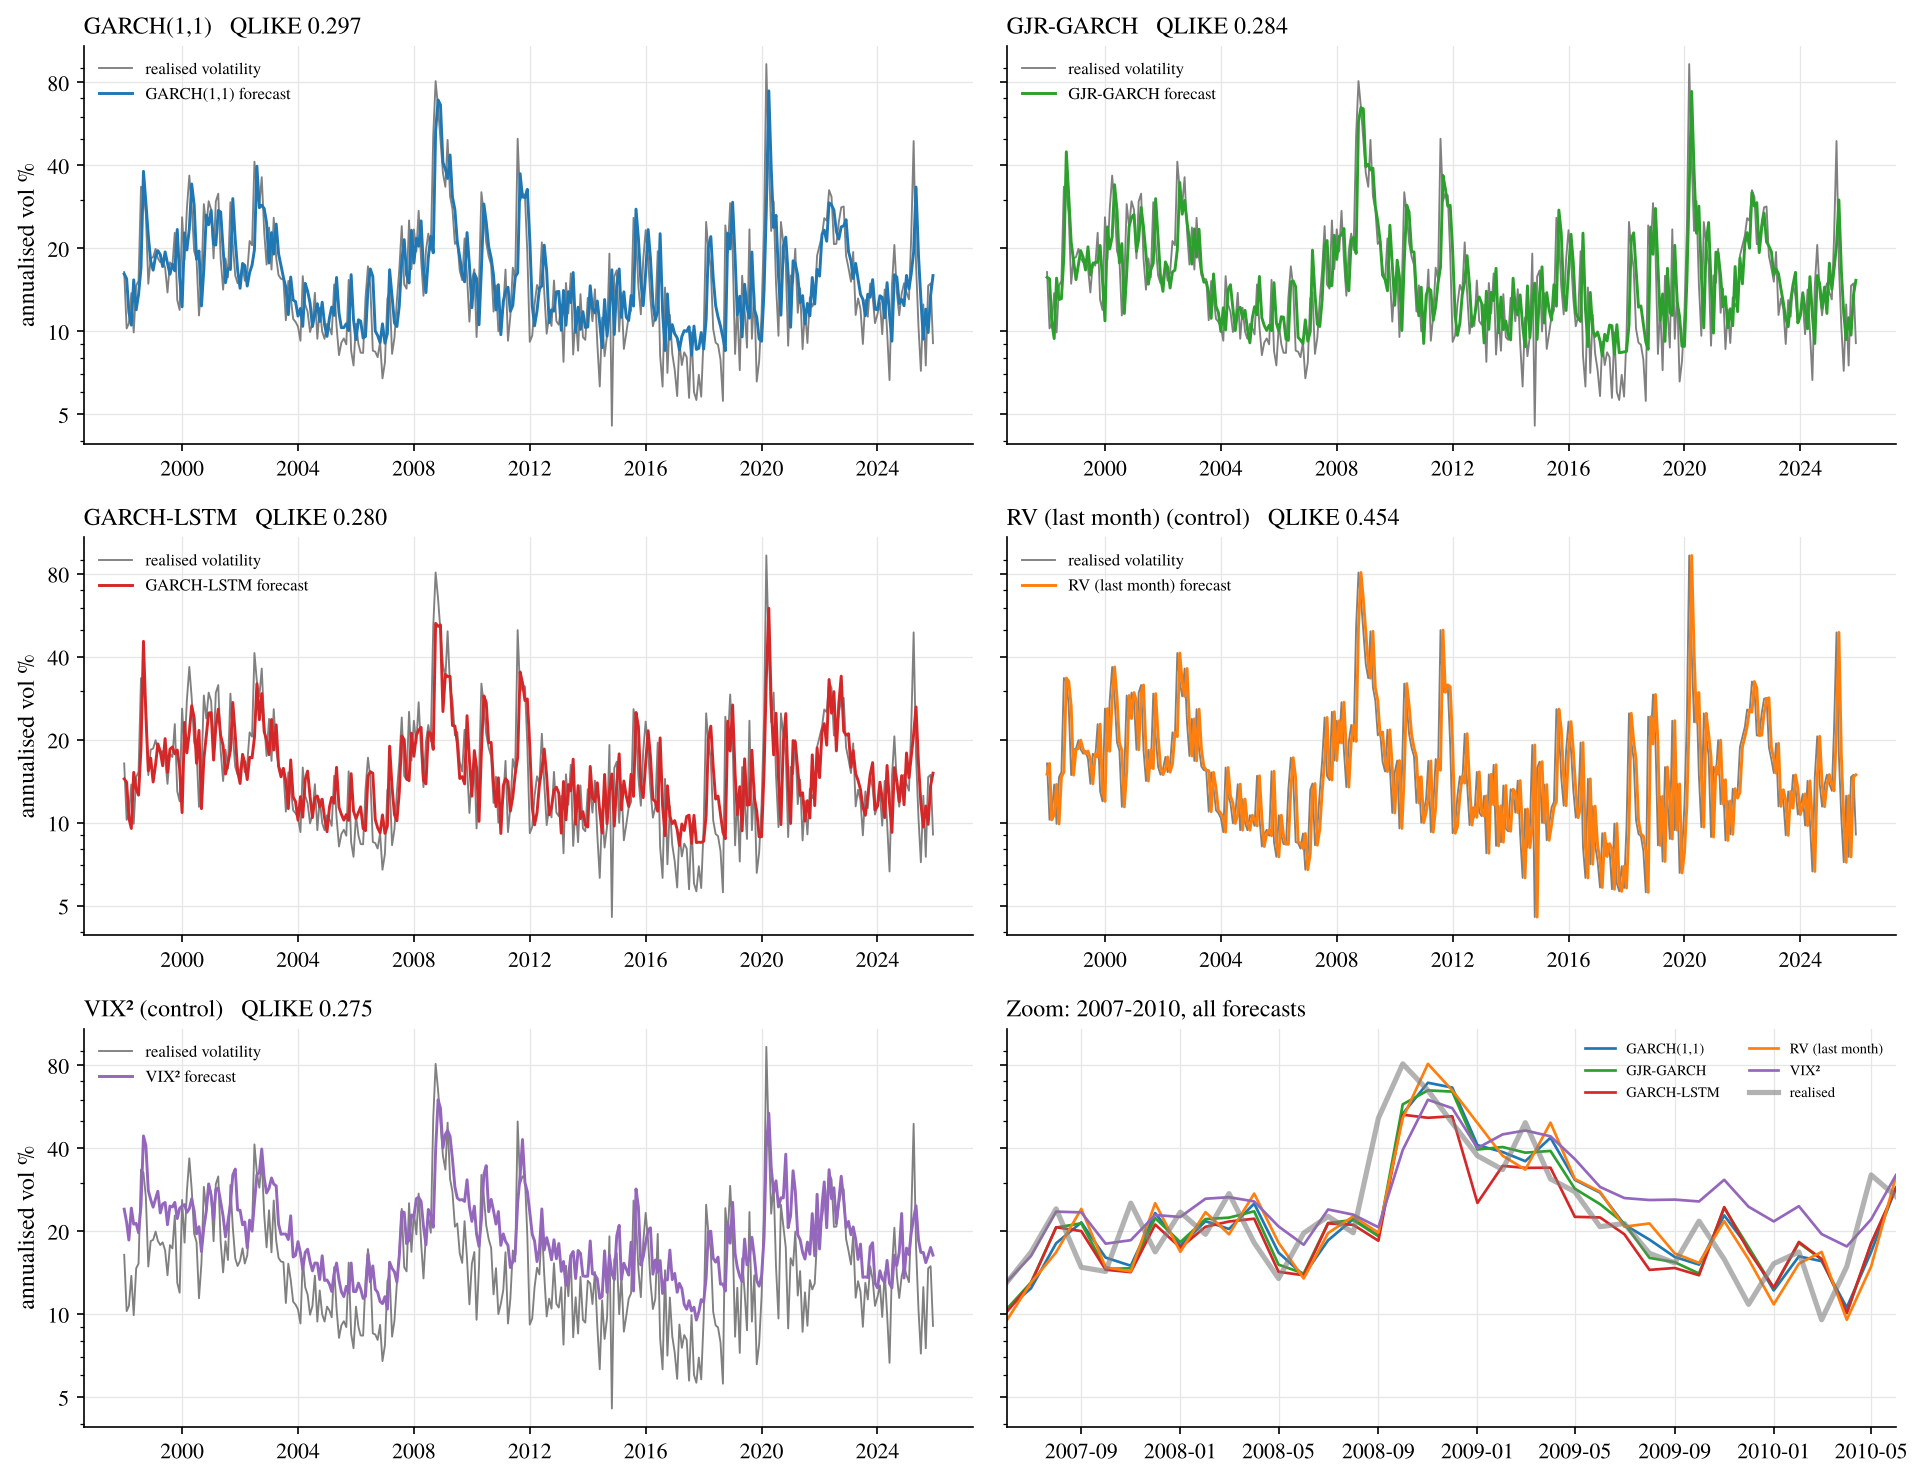
\includegraphics[width=\textwidth]{figs/fig02_forecasts_vs_realised.png}
\caption{Next-month volatility forecasts (coloured) against the realised volatility of the month forecast (grey), annualised, log scale, 1998--2025. Last panel: all forecasts during 2007--2010.}
\label{fig:forecasts}
\end{figure}

\FloatBarrier
\subsection{Portfolio construction: the timing rule as a portfolio optimisation}
\paragraph{Theory.} A mean--variance investor with risk aversion $\gamma$ who splits wealth between the market and cash chooses the exposure
\begin{equation}\label{eq:mv}
\max_w\ \Bigl(w\,\mu_t-\frac{\gamma}{2}w^2\sigma_t^2\Bigr)\quad\Longrightarrow\quad w_t=\frac{\mu_t}{\gamma\,\sigma_t^2},
\end{equation}
where $\mu_t$ and $\sigma_t^2$ are the expected excess return and the variance of the market in month $t$. One could time the expected return, the variance, or both. Volatility timing treats $\mu$ as constant and times only the variance, which is optimal if variance is forecastable and the expected return is not (Section~\ref{sec:why} tests this). With $\mu$ constant, eq.~\eqref{eq:mv} becomes $w_t=c/\sigma_t^2$, where the constant $c=\mu/\gamma$ absorbs the unknown premium and the risk aversion; in practice $\sigma_t^2$ is replaced by its forecast $\hat v_t$.

\paragraph{The rule.} Exposure to the market in month $t$ is
\begin{equation}\label{eq:rule}
w_t=\min\Bigl(\frac{c_t}{\hat v_t},\ 1.5\Bigr).
\end{equation}
Doubling the expected variance halves the position. The scale $c_t$ is a target variance: the rule holds full exposure ($w_t=1$) when the forecast equals the target, less above it, and up to 1.5 below it. The cap of 1.5 (at most 50\% leverage) follows Moreira and Muir (2017, Table V).

\paragraph{Setting $c$ in real time.} Every January we choose $c_t$ so that the capped timed strategy would have had the same volatility as buy and hold over all past months $s$ before January:
\begin{equation}\label{eq:c}
\operatorname{sd}\Bigl[\min\bigl(c_t/\hat v_s,\,1.5\bigr)\,f_s\Bigr]=\operatorname{sd}\bigl[f_s\bigr],\qquad s=\text{all months before January of the current year},
\end{equation}
where sd is the standard deviation. This needs at least 24 months of past forecasts; because of the cap, $c$ is found numerically (Brent's method). Only past data enter. Moreira and Muir (2017) instead pick one $c$ on the full sample, which no investor could have done (Appendix~\ref{app:buildup}). Because $c$ is matched to each forecast's own history, a forecast that is too high or too low on average gets a proportionally larger or smaller $c$: only the variation of a forecast matters for the portfolio, which is why the controls can be compared with the models at all.

For RV, GARCH(1,1) and \VIX, the past forecasts in eq.~\eqref{eq:c} are the forecasts that were actually made in each earlier year. For GJR-GARCH and the GARCH-LSTM, the training run solves the same equation each January on the forecast path that the newly fitted model produces when it re-filters all earlier data, and then holds $c$ fixed for the year. Both use only past data. To check that this difference does not matter, we passed the GJR and GARCH-LSTM forecasts through the first procedure as well: $c$ is on average 5\% to 7\% lower, the exposures are almost identical (correlation 0.997 to 0.999) and the Sharpe ratio changes by at most 0.002. For the three models the implied target volatility $\sqrt{12c_t}$ (the annualised volatility that $c_t$ corresponds to) is about 12\% a year in 1998 and about 14\% by 2025 (18--23\% for \VIX).

\begin{figure}[htbp]
\centering
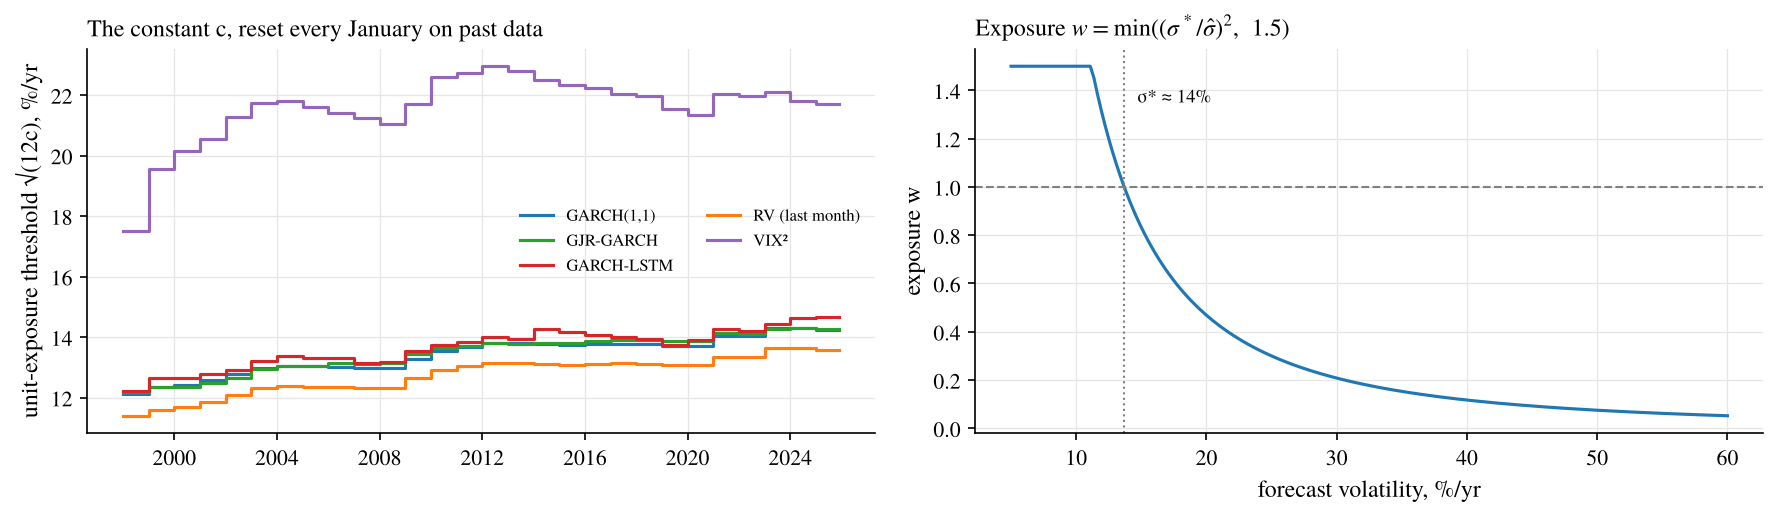
\includegraphics[width=\textwidth]{figs/fig02_timing_rule.png}
\caption{Left: the threshold volatility $\sqrt{12c_t}$ implied by the scale $c_t$, reset every January on past data. Right: the exposure $w_t=\min(c_t/\hat v_t,1.5)$ as a function of the forecast volatility $\sqrt{12\hat v_t}$, for a typical threshold.}
\label{fig:rule}
\end{figure}

\paragraph{Trading, costs and financing.} The portfolio is rebalanced at each month end. Between rebalances the position drifts with the market: an exposure $w_{t-1}$ chosen at the start of month $t-1$ has become, by its end,
\begin{equation}\label{eq:drift}
w^{\text{drift}}_{t-1}=w_{t-1}\,\frac{1+r^f_{t-1}+f_{t-1}}{1+r^f_{t-1}+w_{t-1}f_{t-1}},
\end{equation}
because the market part grew at the market's return and the whole portfolio at the portfolio's return. Costs are paid on the change from this drifted position, so the monthly net excess return is
\begin{equation}\label{eq:net}
z_t=w_t f_t-\kappa\,\bigl|w_t-w^{\text{drift}}_{t-1}\bigr|,\qquad\kappa=0.001\ (10\text{ bp}),
\end{equation}
following Moreira and Muir (2017, Table IV). Cash earns the risk-free rate and leverage is financed at the same rate (no spread). The timed rules hold more than full exposure in 41\% to 44\% of months and borrow on average about 0.16 of capital, so a 1\% a year borrowing spread would cost about 0.16\% a year.

\FloatBarrier
\subsection{Decision-focused training of the forecast (Q3)}\label{sec:dec}
The same variance model is trained in two ways, with the train and validation blocks of Section~\ref{sec:design}:
\begin{itemize}
\item \textbf{Acc} (accuracy, objective A): the quasi-likelihood used for GARCH above, the usual way to fit a variance model: minimise $\frac1D\sum_d(\log h_d+r_d^2/h_d)$ over the training days.
\item \textbf{Dec} (decision, objective B): the investor's utility of the timed portfolio after costs over the training months,
\begin{equation}\label{eq:utility}
\max\ \frac1M\sum_{t=1}^{M} z_t-\frac{\gamma}{2}\,\frac1M\sum_{t=1}^{M} z_t^2,\qquad\gamma=5,
\end{equation}
over the $M$ training months, where $z_t$ is the net return of eq.~\eqref{eq:net} with the exposure $w_t=\min(c_t/\hat v_t,1.5)$ of eq.~\eqref{eq:rule}: the trading rule, its cap and its costs are inside the loss. Inside the loss, $c_t$ is recalibrated every January on the model's own earlier path exactly as at deployment (eq.~\eqref{eq:c}), so the network is trained for the rule it trades. Because $c$ is re-matched to the factor's volatility, Dec cannot win by taking more risk; it can only change when exposure is high or low. There is no closed form for $c$ once the cap binds, so it is found numerically; the optimiser still needs to know how $c$ moves when a forecast moves, and this derivative is obtained from the implicit function theorem applied to eq.~\eqref{eq:c}. Dec starts from the selected Acc model, is trained by Adam (up to 300 steps) and keeps the step with the best utility on the validation block; if no step improves on it, Dec stays equal to Acc.
\end{itemize}
Two models are trained, chosen on theoretical grounds: GJR-GARCH, with few parameters, as a control (Acc and Dec should give similar portfolios), and the flexible GARCH-LSTM (five seeds, each trained separately, forecasts averaged), where the objective has room to matter. Both are trained on all six factors. A decision-trained forecast is judged by the decision: (1) the realised value of its own objective out of sample and (2) the net Sharpe ratio of the timed factor. QLIKE is only a diagnostic of what decision training costs in accuracy. Note that Dec cannot see the level of a forecast (multiplying all forecasts by a constant multiplies $c$ by the same constant), so it has no reason to stay calibrated. One approximation remains in both objectives: the monthly forecast is the one-day forecast carried 21 days forward with eq.~\eqref{eq:monthly}.

\subsection{Benchmarks and performance metrics}
\paragraph{Baseline benchmark (S\&P 500).} The course asks for the S\&P 500 as the baseline. Our data do not contain the S\&P 500 index itself, so the baseline is buy and hold of the CRSP value-weighted US market (Ken French Mkt-RF plus the T-bill rate), with exposure always equal to 1 and no trading costs. This index contains every S\&P 500 stock, is dominated by them by market capitalisation, and moves almost one for one with it; it is the standard market proxy in the volatility-timing literature. We refer to it as ``buy and hold'' or ``the market'' throughout. Section~\ref{sec:otherbench} adds two further passive benchmarks: an equal-weighted portfolio of the six factors and an equal-weighted portfolio of the course CRSP stocks.

\paragraph{Metrics.} Monthly returns are annualised as follows (all net of costs):
\begin{itemize}
\item \textit{Annualised return}: the compound annual growth rate, CAGR $=W^{12/N}-1$, where $W$ is the final value of \$1 invested (total return, $z_t+r^f_t$) and $N$ the number of months; and the arithmetic mean of monthly excess returns, $12\bar z$, with $\bar z$ the average of $z_t$;
\item \textit{Annualised standard deviation}: $\sqrt{12}\,\operatorname{sd}(z_t)$;
\item \textit{Sharpe ratio}: $\sqrt{12}\,\bar z/\operatorname{sd}(z_t)$; \textit{Sortino ratio}: $\sqrt{12}\,\bar z/DD$, where the downside deviation $DD$ is the square root of the average of $\min(z_t,0)^2$, so only losses count as risk;
\item \textit{Maximum drawdown}: the largest fall of month-end total-return wealth from its previous peak, including the starting value of \$1; also reported ``at equal volatility'', after rescaling the timed series to buy and hold's volatility (a diagnostic, not a traded strategy);
\item \textit{Calmar ratio} (CAGR/$|$max DD$|$), \textit{certainty-equivalent return} CER $=12\bigl(\bar z-\frac{\gamma}{2}\operatorname{var}(z_t)\bigr)$ with $\gamma=5$, CAPM alpha and beta against the market, and \textit{vol of vol} (the standard deviation of the 12-month rolling volatility).
\end{itemize}

\paragraph{Decomposing the Sharpe ratio.} Let $x_t=w_t/\bar w$ be the exposure divided by its average, so that $x_t$ averages 1. Before costs the timed return $w_tf_t$ is proportional to $x_tf_t$, which has the same Sharpe ratio, and the ratio of the two Sharpe ratios splits exactly into two factors:
\begin{equation}\label{eq:mtvt}
\frac{\text{Sharpe}_{\text{timed}}}{\text{Sharpe}_{\text{buy and hold}}}=\underbrace{\frac{\operatorname{mean}(x_tf_t)}{\operatorname{mean}(f_t)}}_{MT\ \text{(mean timing)}}\times\underbrace{\frac{\operatorname{sd}(f_t)}{\operatorname{sd}(x_tf_t)}}_{VT\ \text{(variance timing)}}.
\end{equation}
VT asks whether the exposure cut risk; MT whether it was high in the months that paid well. Above 1 is good for both.

\paragraph{Statistical inference.} Differences against buy and hold are tested with a \textbf{paired circular block bootstrap} (Künsch, 1989; Politis and Romano, 1992): 12-month blocks, 5,000 resamples, the same blocks for both strategies so their correlation is kept; the 95\% interval is the estimate $\pm$ the 95th percentile of the absolute bootstrap error. Sharpe differences are also tested with the \textbf{Ledoit and Wolf (2008) delta-method HAC test} (Bartlett weights, Newey and West, 1987, 5 lags), and families of comparisons with the \textbf{Romano and Wolf (2005) stepdown adjustment}.

%======================================================================
\section{Performance evaluation}
\FloatBarrier
\subsection{Portfolio value over the backtesting period}
Figure~\ref{fig:growth} shows the value of \$1 invested in January 1998 in each portfolio, as total return net of costs. Over the 28 years the market (our S\&P 500 proxy) grows \$1 to \$12.31, the accuracy-trained timed portfolios to between \$9.46 (GJR-GARCH) and \$9.90 (GARCH-LSTM), the decision-trained GARCH-LSTM to \$9.65, and cash to \$1.78. The curves tell the main story of the project. The timed portfolios lag in strong bull markets (1998--2000, 2016--2021, 2023--2025), when they hold the market at well below full exposure after volatile spells, and they fall much less in slow crashes: in late 2002 and early 2009 buy and hold falls back below its starting value (to \$0.89 and \$0.96), while the timed portfolios stay near \$1.0 in 2002 and between \$1.4 and \$1.5 in 2009. Because the timed portfolios run at about 11\% volatility against 16\%, lower terminal wealth with a higher Sharpe ratio is the expected result: they deliver more return per unit of risk, not more return.

Figure~\ref{fig:volgrowth} adds the 12-month rolling volatility and the drawdown. The timed portfolios keep their volatility between about 4\% and 20\% while buy and hold swings between about 4\% and 31\%, and their drawdowns in 2002 and 2009 are about half as deep.

\begin{figure}[htbp]
\centering
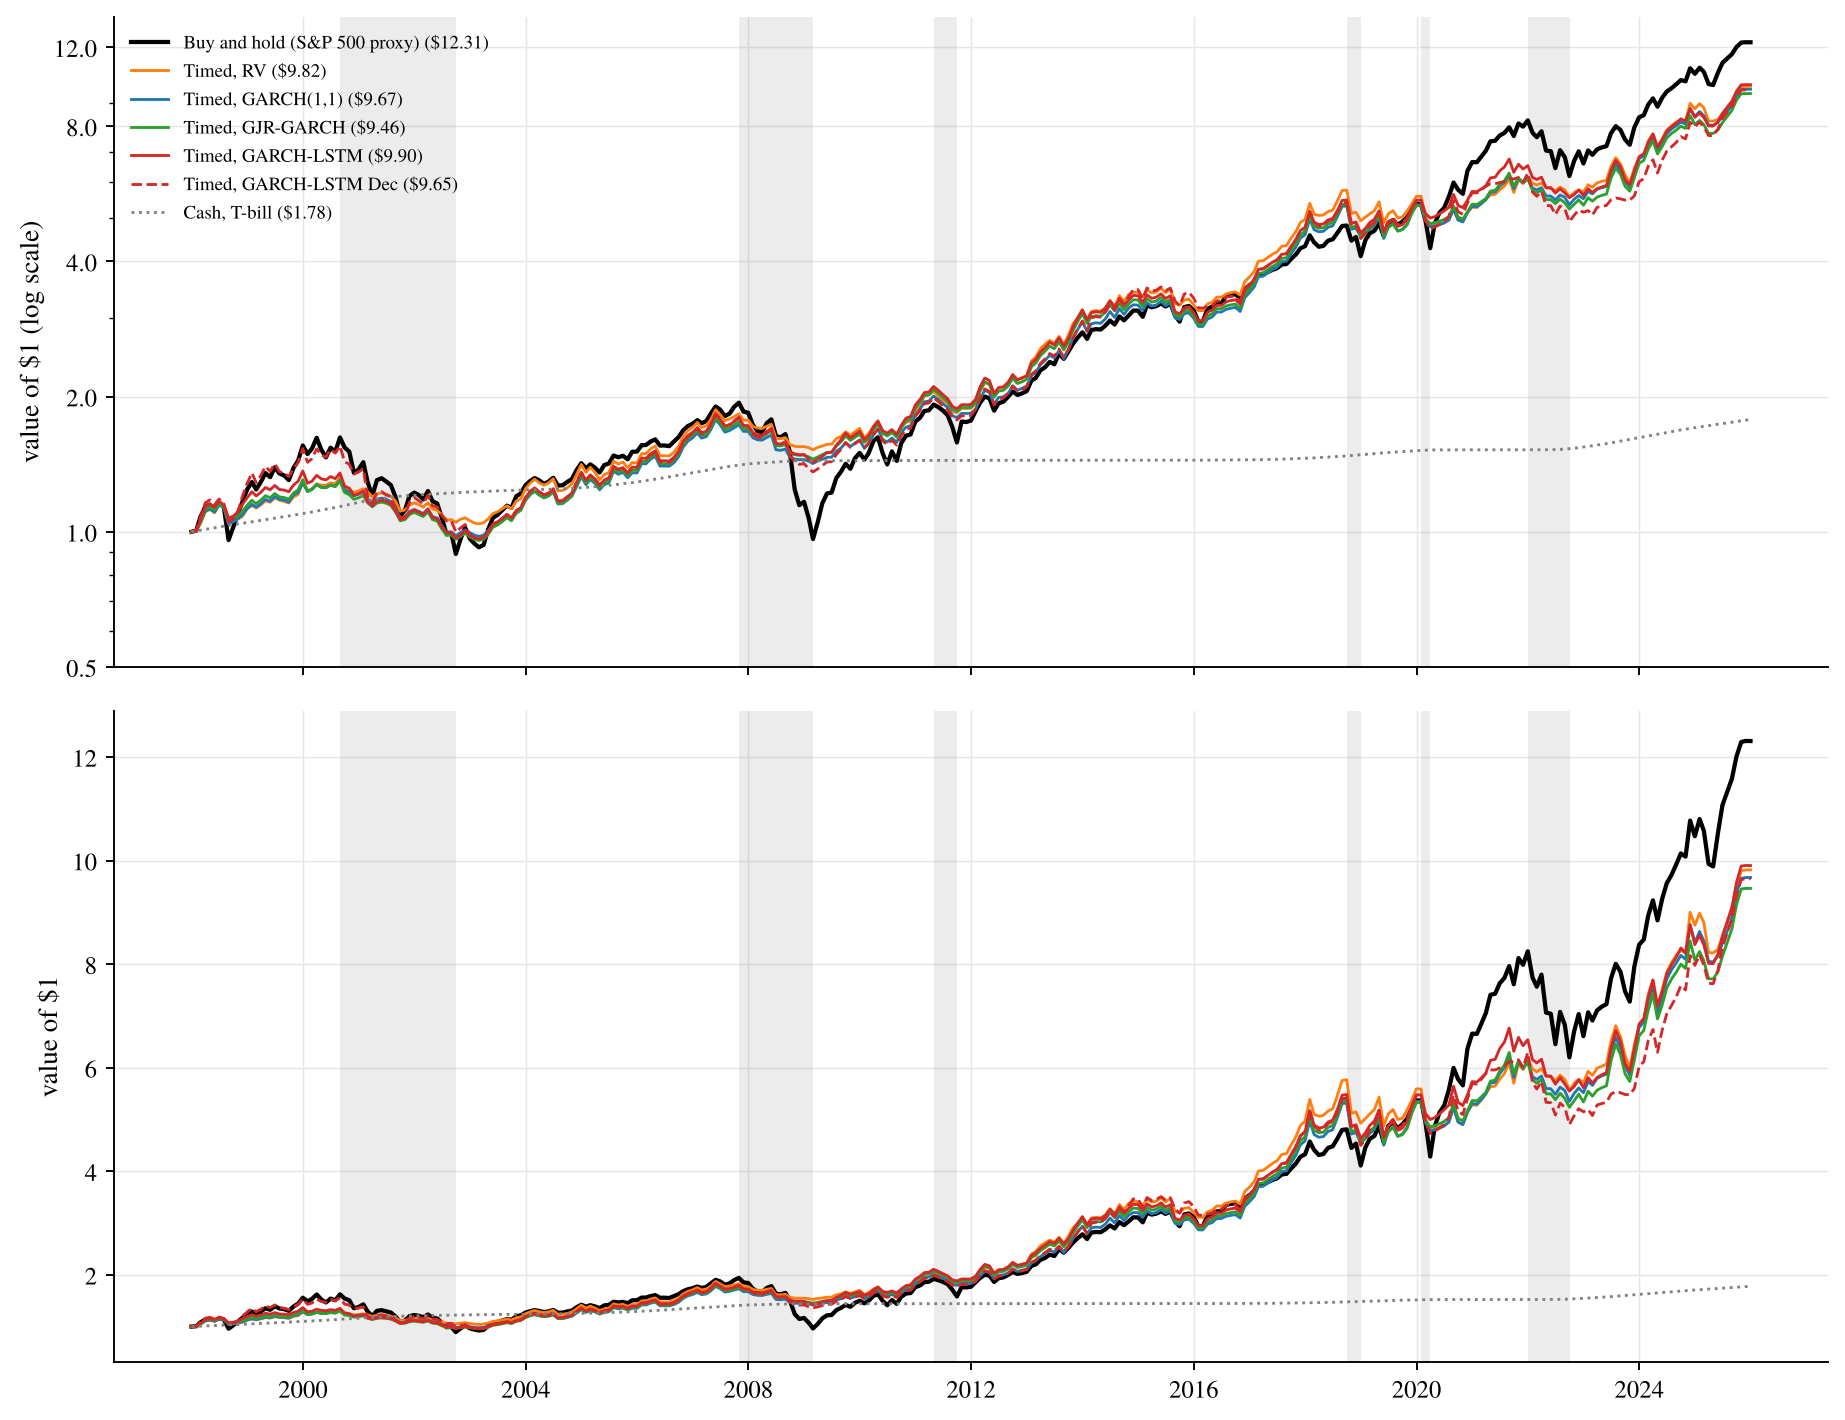
\includegraphics[width=0.93\textwidth]{figs/fig_growth.png}
\caption{Value of \$1 invested in January 1998, total return (excess return plus T-bill rate) net of 10 bp costs, log scale (top) and linear scale (bottom). Benchmark: buy and hold of the CRSP value-weighted US market (S\&P 500 proxy). ``Dec'' is the decision-trained GARCH-LSTM (Section~\ref{sec:q3}). Grey bands: the six crisis episodes.}
\label{fig:growth}
\end{figure}

\begin{figure}[htbp]
\centering
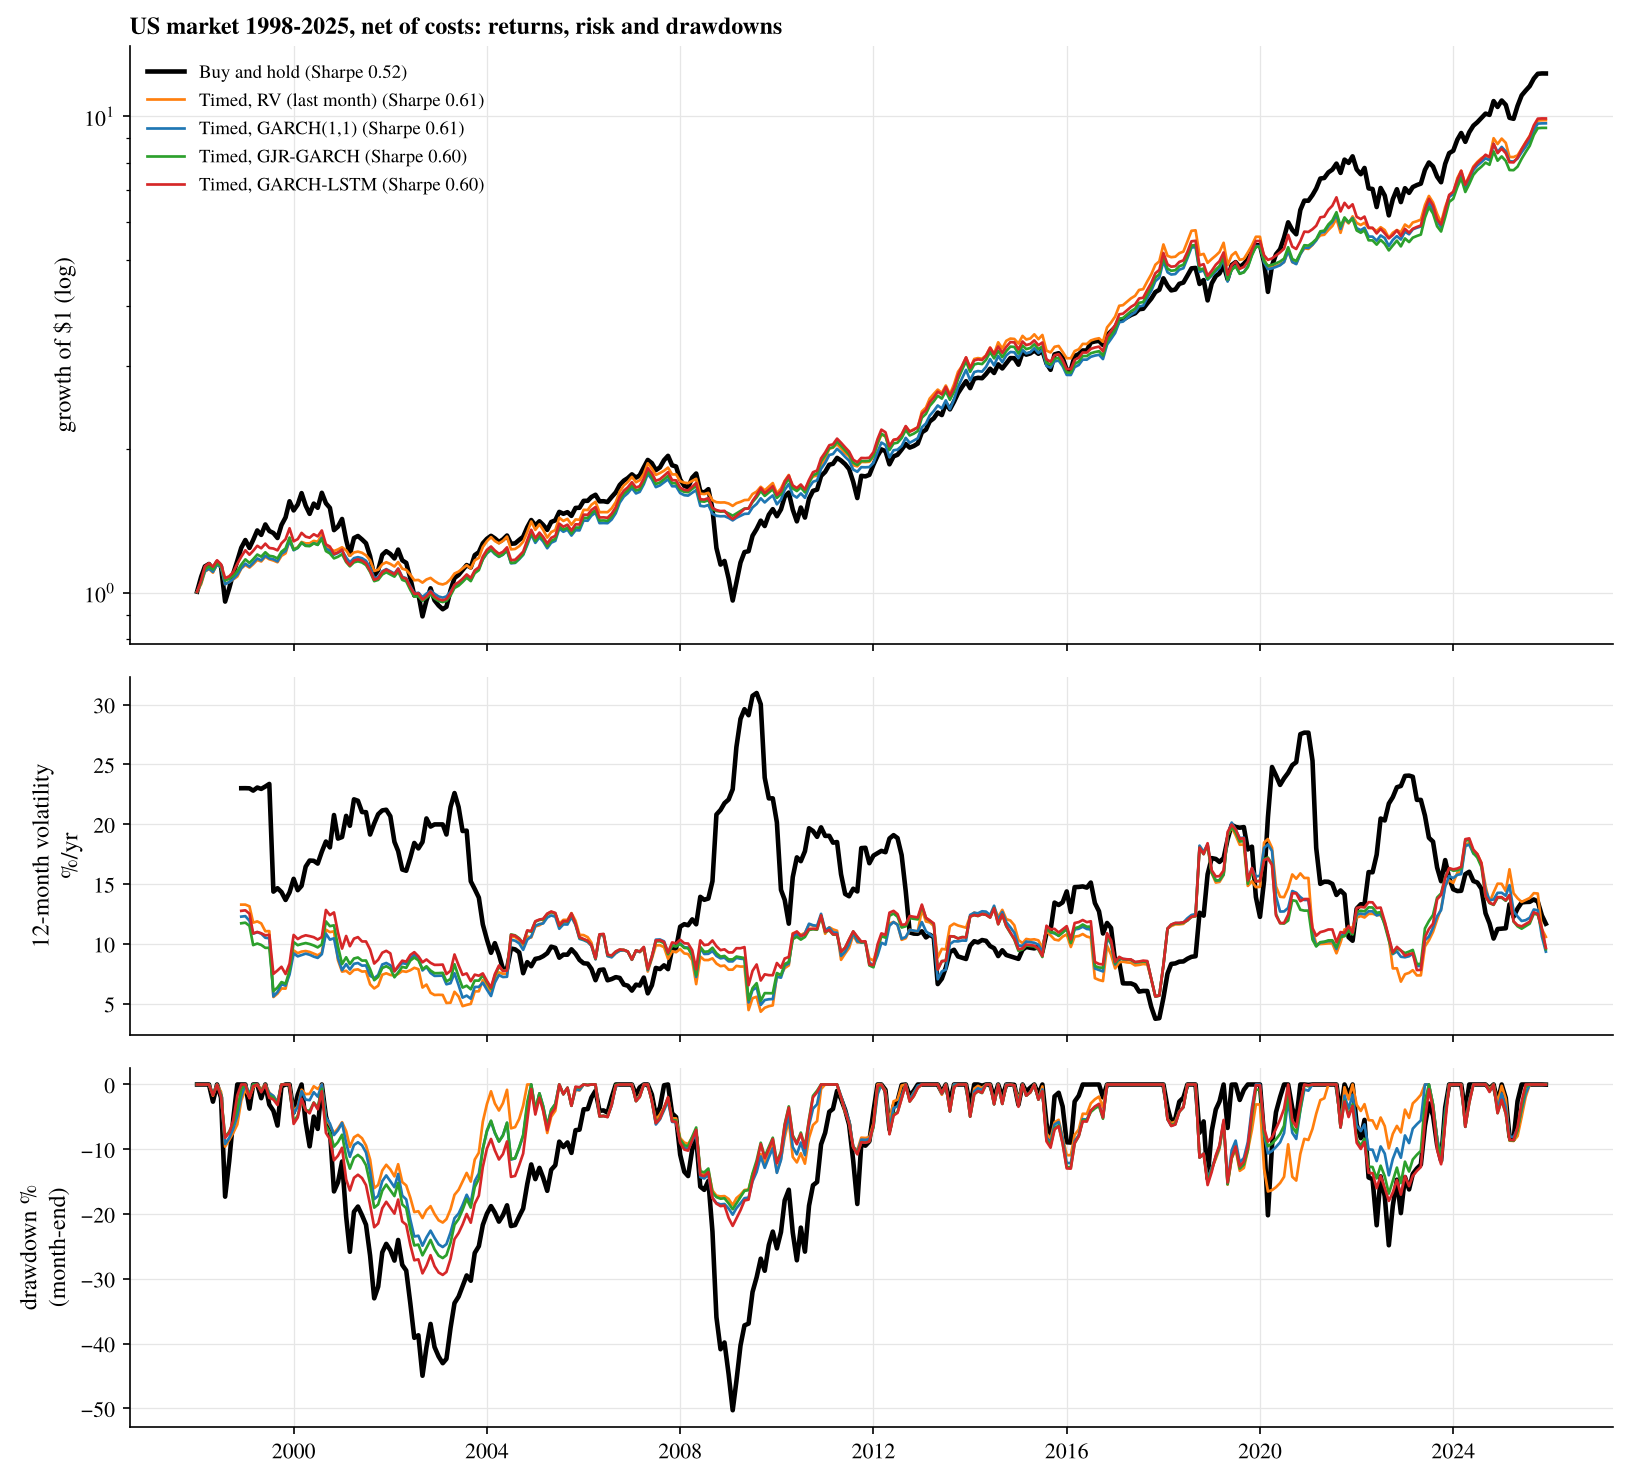
\includegraphics[width=0.85\textwidth]{figs/fig03_growth_vol_drawdown.png}
\caption{Growth of \$1 (log), 12-month rolling volatility and month-end drawdown, 1998--2025, net of costs.}
\label{fig:volgrowth}
\end{figure}

\FloatBarrier
\subsection{Performance table against the benchmark}
Table~\ref{tab:perf} reports the required metrics for the full test period.

Every accuracy-trained timed portfolio beats the S\&P 500 proxy on every risk-adjusted measure: Sharpe ratio 0.60--0.61 against 0.52, Sortino ratio 0.89--0.92 against 0.75, Calmar ratio 1.6 to 2.1 times as high, and a worst drawdown cut from $-$50\% to between $-$21\% and $-$29\%. They give up 0.8 to 1.0 points of compound annual return (1.4 to 1.6 points of mean excess return) for about 30\% less volatility, with a market beta of 0.53 to 0.58. The CAPM alpha is about 2\% a year but not significant at 5\% ($t$ between 1.6 and 1.7). Among the accuracy-trained forecasts RV, the least accurate, has the best Sharpe ratio and the smallest drawdown; GJR-GARCH and the GARCH-LSTM have the lowest Sharpe ratio (0.597). The GARCH-LSTM holds the most market on average (0.92), so it ends with the most wealth of the four but also has the deepest drawdown. Sections~\ref{sec:q2}--\ref{sec:why} explain the ordering. The decision-trained GARCH-LSTM is the weakest timed portfolio on the market (Sharpe 0.537, worst drawdown $-$37.9\%).

Figure~\ref{fig:years} shows calendar-year returns. The accuracy-trained timed portfolios beat the market in 11 to 14 of the 28 years (the decision-trained one in 12), mainly in down years (2000--2002, 2008, 2022), and lag in strong up years.

\begin{table}[htbp]
\centering\small
\caption{Portfolio performance, US market, January 1998 -- December 2025 (336 months), net of 10 bp costs.}\label{tab:perf}
\begin{adjustbox}{max width=\linewidth}\begin{tabular}{@{}lcccccc@{}}
\toprule
 & Buy and hold & \multicolumn{4}{c}{Timed, accuracy-trained forecast} & Timed\\
\cmidrule(lr){3-6}
 & (S\&P 500) & RV & GARCH & GJR & GARCH-LSTM & LSTM Dec\\
\midrule
Ann.\ return (CAGR), \% & \textbf{9.38} & 8.50 & 8.44 & 8.36 & 8.53 & 8.43\\
Ann.\ excess return (mean), \% & \textbf{8.22} & 6.73 & 6.68 & 6.61 & 6.81 & 6.89\\
Ann.\ std.\ deviation, \% & 15.93 & 11.00 & \textbf{10.99} & 11.07 & 11.40 & 12.84\\
Sharpe ratio & 0.516 & \textbf{0.612} & 0.608 & 0.597 & 0.597 & 0.537\\
Maximum drawdown, \% & $-$50.3 & \textbf{$-$21.3} & $-$25.1 & $-$26.8 & $-$29.4 & $-$37.9\\
Sortino ratio & 0.748 & \textbf{0.919} & 0.909 & 0.891 & 0.889 & 0.781\\
Calmar ratio & 0.19 & \textbf{0.40} & 0.34 & 0.31 & 0.29 & 0.22\\
Max DD at market vol, \% & $-$50.3 & \textbf{$-$32.0} & $-$36.9 & $-$39.8 & $-$41.8 & $-$46.2\\
CER ($\gamma=5$), \% p.a. & 1.87 & \textbf{3.71} & 3.66 & 3.54 & 3.56 & 2.77\\
CAPM beta & 1.00 & 0.53 & 0.55 & 0.55 & 0.58 & 0.68\\
CAPM alpha, \% ($t$) & -- & \textbf{2.37} (1.74) & 2.15 (1.67) & 2.09 (1.57) & 2.05 (1.59) & 1.33 (1.03)\\
Worst month, \% & $-$17.2 & $-$11.5 & $-$11.5 & $-$11.5 & $-$11.5 & $-$13.6\\
Value of \$1 at end, \$ & \textbf{12.31} & 9.82 & 9.67 & 9.46 & 9.90 & 9.65\\
Average exposure & 1.00 & 0.86 & 0.88 & 0.89 & 0.92 & 0.96\\
Exposure traded per year & 0.00 & 3.79 & 3.28 & 3.53 & 3.59 & 3.49\\
\bottomrule
\end{tabular}\end{adjustbox}
\par\smallskip\parbox{\textwidth}{\footnotesize Returns are total returns (CAGR) or excess returns over the T-bill (mean), annualised from monthly data; drawdowns are on month-end wealth. Alpha $t$-statistics use Newey--West standard errors (5 lags). Cash (T-bill) CAGR: 2.08\%. Best value in each row in bold. LSTM Dec: decision-trained GARCH-LSTM (Section~\ref{sec:q3}).}
\end{table}

\begin{figure}[htbp]
\centering
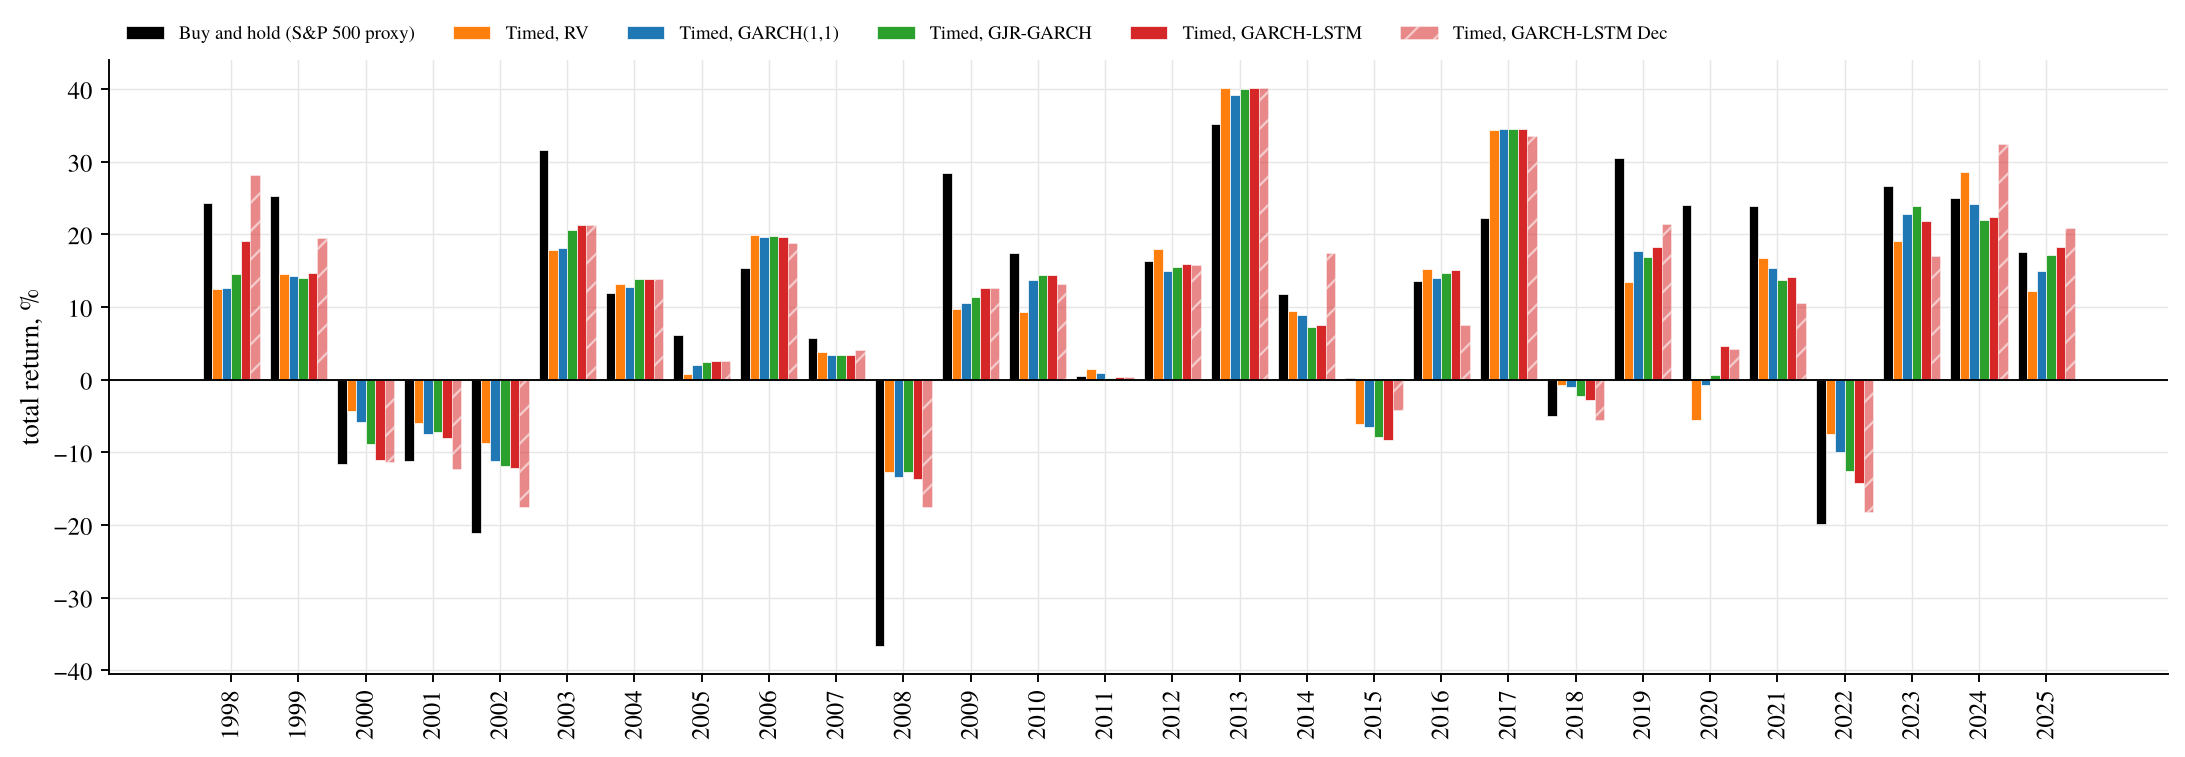
\includegraphics[width=\textwidth]{figs/fig_years.png}
\caption{Calendar-year total returns, net of costs, 1998--2025.}
\label{fig:years}
\end{figure}

\FloatBarrier
\subsection{Sub-periods}
The gain is concentrated in 1998--2015, a period with two deep bear markets, when the timed Sharpe ratio is 0.45--0.50 against 0.35 and the timed portfolios roughly match the market's compound return with about 35\% less volatility. Over 2016--2025 the accuracy-trained timed portfolios are level with or slightly behind buy and hold on the Sharpe ratio (0.78--0.83 against 0.82) and earn 2 to 3 points a year less (Table~\ref{tab:sub}). Figure~\ref{fig:rolling} shows the same pattern in the rolling 36-month Sharpe ratio: the timed portfolios are ahead in and after the 2000--2002 and 2008--2009 bear markets and behind in the long bull market of the 2010s.

\begin{table}[htbp]
\centering\small
\caption{Performance by sub-period, net of costs: CAGR (\%), annualised volatility (\%), Sharpe ratio and maximum drawdown within the period (\%).}\label{tab:sub}
\setlength{\tabcolsep}{4pt}
\begin{adjustbox}{max width=\linewidth}\begin{tabular}{@{}lcccccccccccc@{}}
\toprule
 & \multicolumn{4}{c}{1998--2015} & \multicolumn{4}{c}{2016--2025} & \multicolumn{4}{c}{2021--2025}\\
\cmidrule(lr){2-5}\cmidrule(lr){6-9}\cmidrule(lr){10-13}
 & CAGR & Vol & SR & MDD & CAGR & Vol & SR & MDD & CAGR & Vol & SR & MDD\\
\midrule
Buy and hold (S\&P 500) & 6.5 & 16.0 & 0.348 & $-$50.3 & 14.7 & 15.7 & 0.824 & $-$24.8 & 13.1 & 15.3 & 0.679 & $-$24.8\\
Timed, RV & 6.7 & 9.9 & 0.499 & $-$21.3 & 11.8 & 12.8 & 0.781 & $-$16.5 & 13.2 & 12.2 & 0.828 & $-$12.1\\
Timed, GARCH(1,1) & 6.3 & 9.9 & 0.460 & $-$25.1 & 12.5 & 12.7 & 0.828 & $-$15.3 & 12.8 & 12.1 & 0.800 & $-$14.0\\
Timed, GJR-GARCH & 6.3 & 10.1 & 0.459 & $-$26.8 & 12.1 & 12.7 & 0.803 & $-$16.8 & 12.0 & 12.3 & 0.734 & $-$16.8\\
Timed, GARCH-LSTM & 6.4 & 10.5 & 0.454 & $-$29.4 & 12.4 & 12.8 & 0.815 & $-$18.0 & 11.6 & 12.5 & 0.695 & $-$18.0\\
Timed, GARCH-LSTM Dec & 6.9 & 12.6 & 0.431 & $-$37.9 & 11.3 & 13.3 & 0.718 & $-$22.1 & 11.1 & 12.1 & 0.681 & $-$22.1\\
\bottomrule
\end{tabular}\end{adjustbox}
\end{table}

\begin{figure}[htbp]
\centering
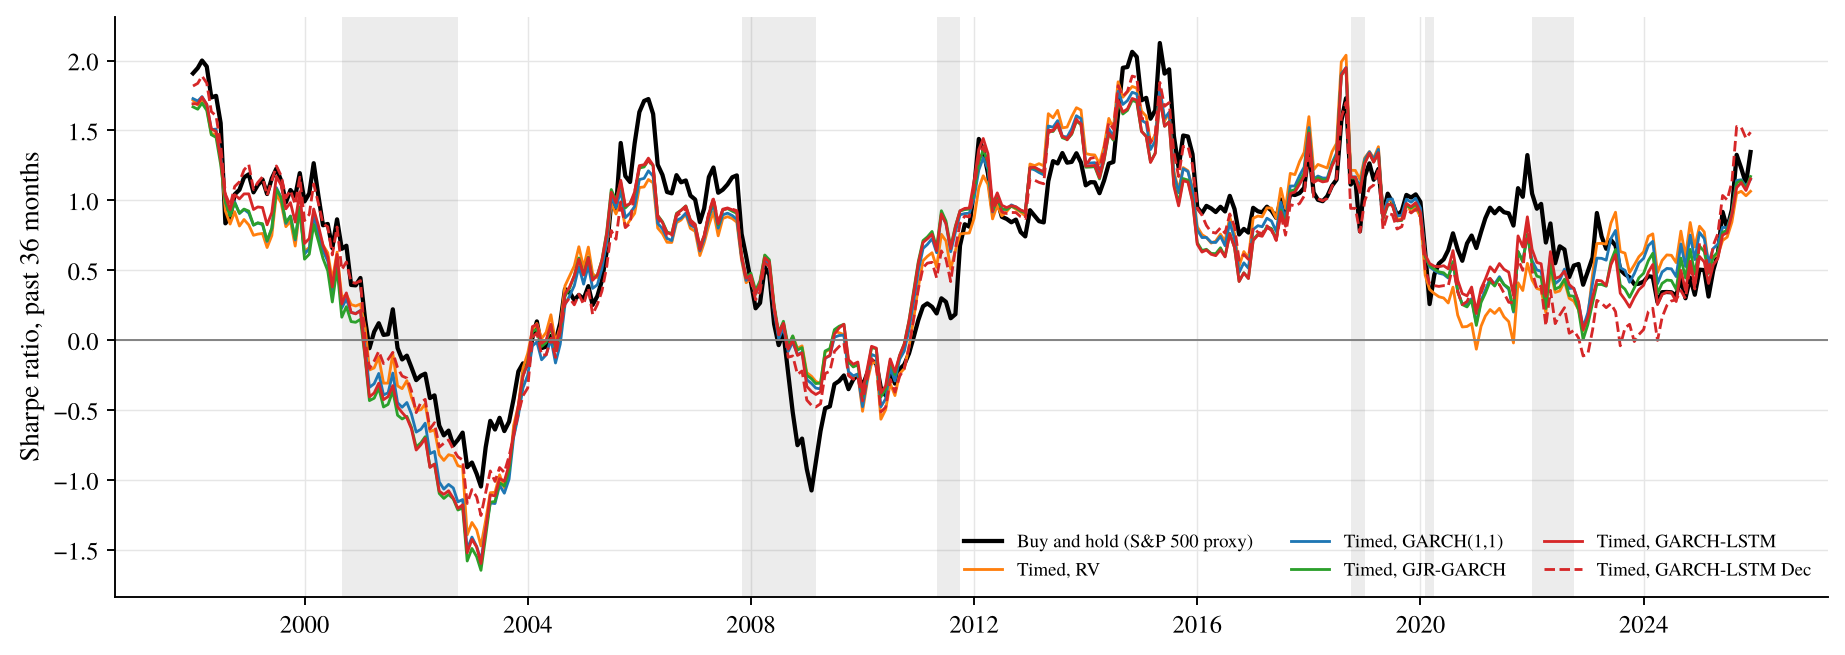
\includegraphics[width=0.9\textwidth]{figs/fig_rolling_sharpe.png}
\caption{Rolling 36-month Sharpe ratio, net of costs.}
\label{fig:rolling}
\end{figure}

\FloatBarrier
\subsection{Crisis episodes}
In five of the six episodes all four timed portfolios lost less than buy and hold, typically about half as much (Table~\ref{tab:crises}, Figure~\ref{fig:crises}). The exception is the sudden Q4 2018 sell-off ($-$14.6\% to $-$15.5\% against $-$14.5\%), which followed a calm summer with high exposure, so the forecast had no time to react. The price of protection is the rebound: in the month after each episode the exposure is only 0.02 to 0.34, so the rules miss much of the recovery (Section~\ref{sec:why}). The GARCH-LSTM and GJR-GARCH lost least in the Covid crash ($-$8.7\% and $-$8.8\%), and the GARCH-LSTM lost most of the timed rules in the dot-com and financial crises ($-$28.4\% and $-$20.3\%).

\begin{table}[htbp]
\centering\small
\caption{Total return over each crisis episode, \%, as traded, net of costs, and the exposure held in the month after the episode.}\label{tab:crises}
\setlength{\tabcolsep}{4.5pt}
\begin{adjustbox}{max width=\linewidth}\begin{tabular}{@{}lccccc|cccc@{}}
\toprule
 & \multicolumn{5}{c|}{Return over the episode, \%} & \multicolumn{4}{c}{Exposure in the month after}\\
Episode & Buy \& hold & RV & GARCH & GJR & LSTM & RV & GARCH & GJR & LSTM\\
\midrule
Dot-com (2000-09 to 2002-09) & $-$45.0 & $-$20.6 & $-$24.9 & $-$25.9 & $-$28.4 & 0.18 & 0.20 & 0.18 & 0.19\\
Financial (2007-11 to 2009-02) & $-$50.3 & $-$16.9 & $-$18.0 & $-$17.6 & $-$20.3 & 0.14 & 0.14 & 0.12 & 0.16\\
Euro (2011-05 to 2011-09) & $-$17.6 & $-$10.2 & $-$10.5 & $-$10.7 & $-$10.8 & 0.19 & 0.20 & 0.17 & 0.19\\
Q4 2018 & $-$14.5 & $-$14.6 & $-$14.6 & $-$15.1 & $-$15.5 & 0.20 & 0.22 & 0.25 & 0.27\\
Covid (2020-02 to 2020-03) & $-$20.2 & $-$13.9 & $-$10.6 & $-$8.8 & $-$8.7 & 0.02 & 0.03 & 0.04 & 0.05\\
Bear 2022 (2022-01 to 2022-09) & $-$24.8 & $-$9.9 & $-$12.6 & $-$14.2 & $-$15.2 & 0.29 & 0.34 & 0.28 & 0.17\\
\bottomrule
\end{tabular}\end{adjustbox}
\end{table}

\begin{figure}[htbp]
\centering
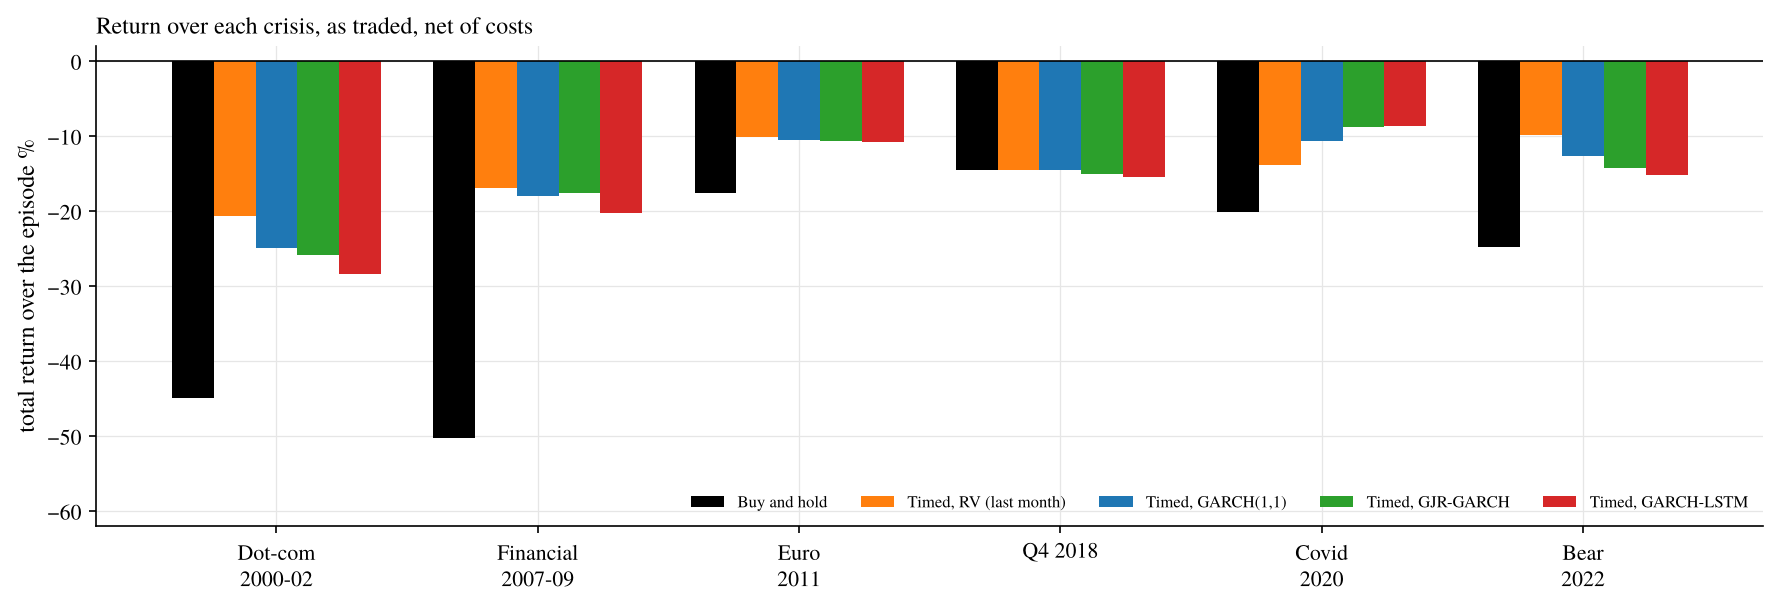
\includegraphics[width=0.85\textwidth]{figs/fig03_crises.png}
\caption{Total return over each crisis episode, as traded, net of costs.}
\label{fig:crises}
\end{figure}

\FloatBarrier
\subsection{Q1: what improves, and is it significant?}
Timing is meant to be a risk tool, so we test five measures, timed minus buy and hold (Table~\ref{tab:q1}, Figure~\ref{fig:improves}).

\begin{table}[htbp]
\centering\small
\caption{Timed minus buy and hold, 1998--2025; block-bootstrap $p$-values in brackets. Positive = better for the timed portfolio. ``Equal vol'': timed returns rescaled after the fact to buy and hold's volatility.}\label{tab:q1}
\begin{adjustbox}{max width=\linewidth}\begin{tabular}{@{}lcccc@{}}
\toprule
 & RV & GARCH(1,1) & GJR-GARCH & GARCH-LSTM\\
\midrule
Sharpe ratio & $+$0.10 (0.48) & $+$0.09 (0.44) & $+$0.08 (0.51) & $+$0.08 (0.48)\\
Sortino ratio & $+$0.17 (0.48) & $+$0.16 (0.45) & $+$0.14 (0.51) & $+$0.14 (0.49)\\
Max DD at equal vol, pts & $+$18.3 (0.10) & $+$13.4 (0.14) & $+$10.6 (0.26) & $+$8.5 (0.35)\\
Vol of vol at equal vol, pts & $+$1.2 (0.09) & \textbf{$+$1.6 (0.03)} & \textbf{$+$1.8 (0.02)} & \textbf{$+$2.1 (0.005)}\\
CER, \% p.a. & $+$1.8 (0.44) & $+$1.8 (0.41) & $+$1.7 (0.44) & $+$1.7 (0.40)\\
Sharpe: Ledoit--Wolf $p$ & 0.49 & 0.47 & 0.53 & 0.50\\
Sharpe: Romano--Wolf $p$ & 0.61 & 0.59 & 0.61 & 0.61\\
\bottomrule
\end{tabular}\end{adjustbox}
\end{table}

\begin{figure}[htbp]
\centering
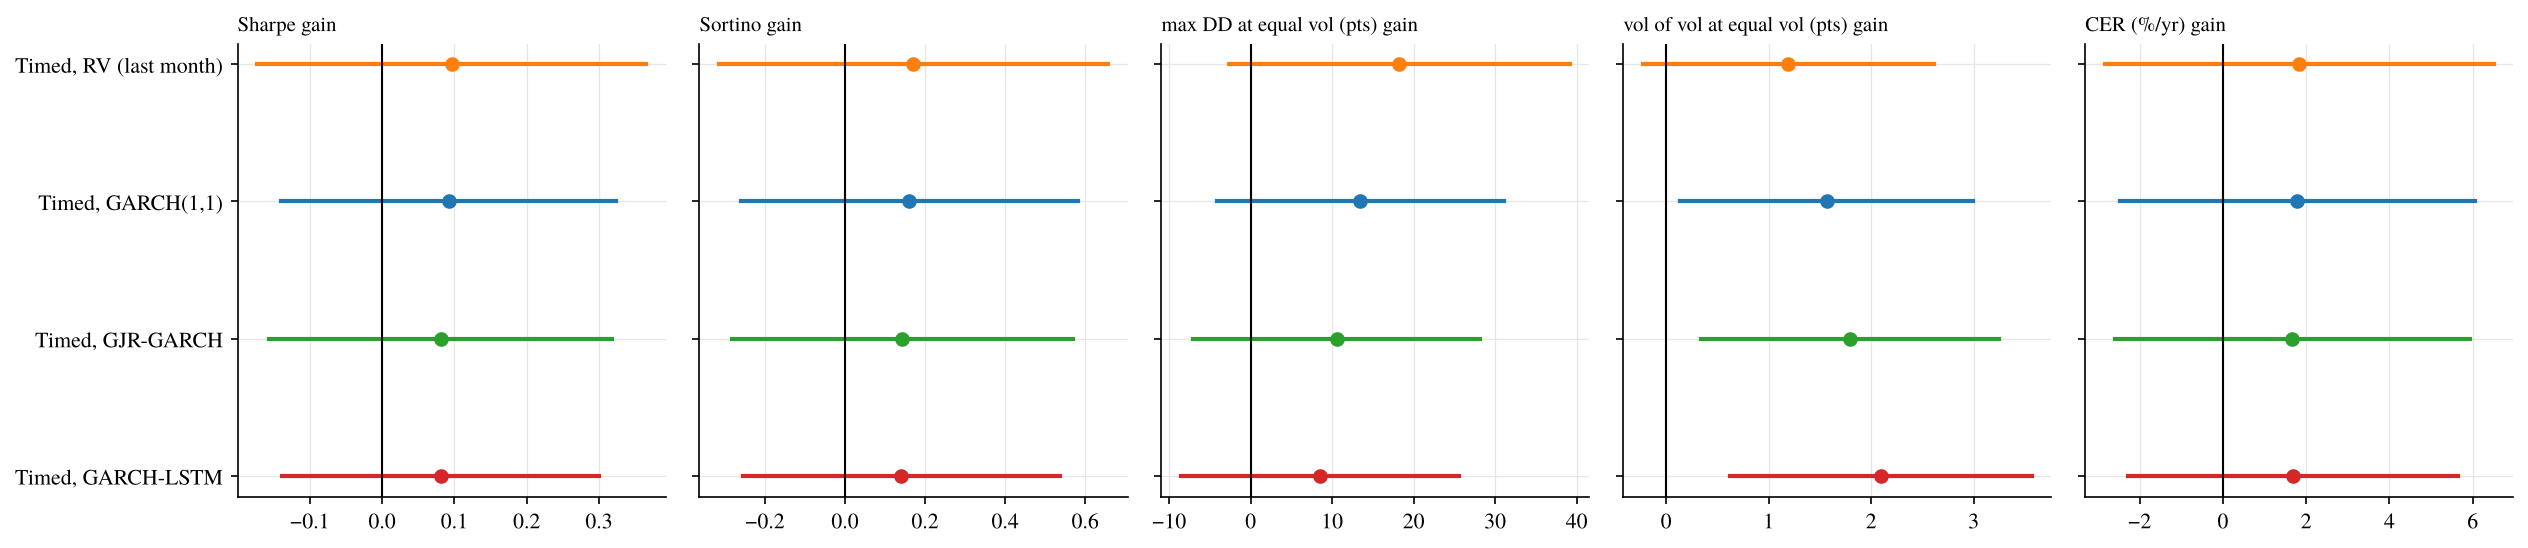
\includegraphics[width=\textwidth]{figs/fig03_what_improves.png}
\caption{What timing improves: timed minus buy and hold, 1998--2025, with 95\% block-bootstrap intervals (right of zero = better).}
\label{fig:improves}
\end{figure}

\begin{itemize}
\item \textbf{Drawdowns.} At equal volatility the timed portfolios' worst drawdown is 8 to 18 points smaller ($-$32\% to $-$42\% against $-$50\%), and as traded it roughly halves. The intervals include zero ($p$ 0.10 to 0.35): with one 28-year history and a handful of crashes, a drawdown difference is hard to prove.
\item \textbf{Steadier risk.} Rescaled to the same volatility, the GARCH(1,1), GJR-GARCH and GARCH-LSTM portfolios have a vol of vol 1.6 to 2.1 points lower than buy and hold (3.7\% to 4.2\% against 5.8\%), with intervals that exclude zero ($p$ 0.005 to 0.033, before adjusting for four rules). This is the only statistically significant improvement, and exactly what an inverse-variance rule is designed to deliver.
\item \textbf{Sharpe ratio.} $+$0.08 to $+$0.10, not significant with either test, before or after the Romano--Wolf adjustment, in any period: $+$0.11 to $+$0.15 in 1998--2015 and $-$0.04 to $+$0.00 in 2016--2025 (Figure~\ref{fig:byperiod}).
\end{itemize}
\textit{Answer to Q1: yes on risk, no on return.} Timing makes the ride smoother; it does not make the investor reliably richer per unit of risk.

\begin{figure}[htbp]
\centering
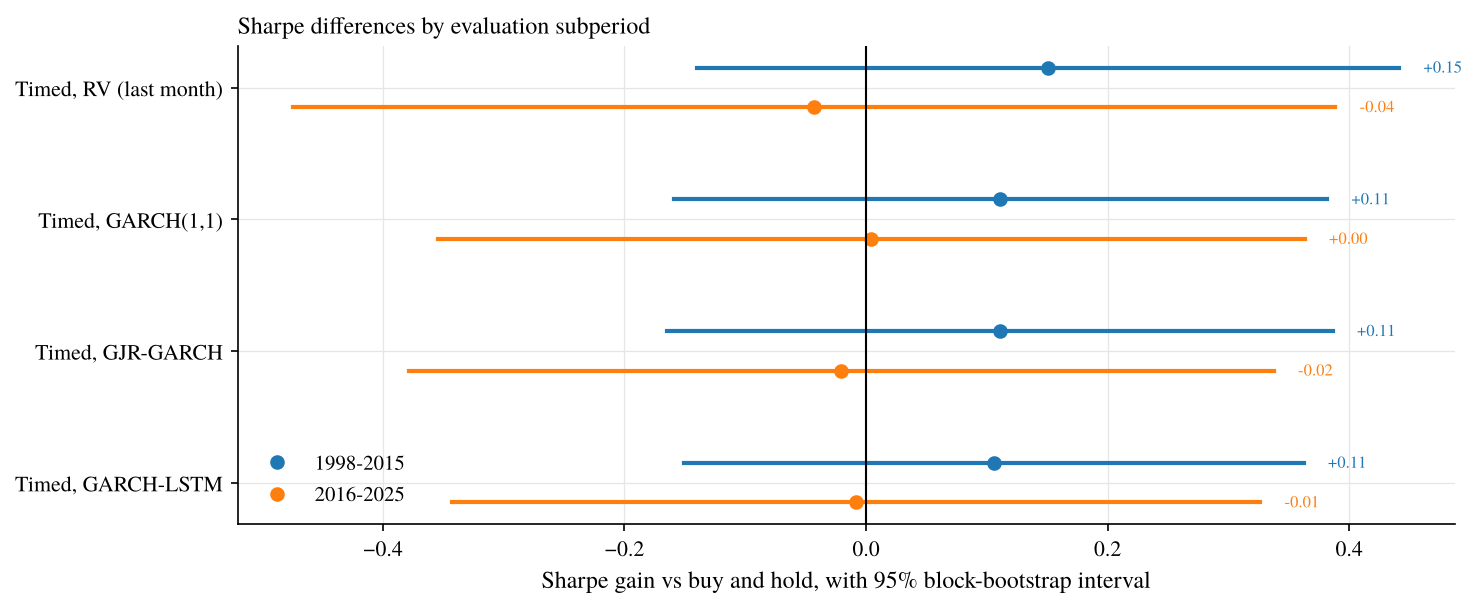
\includegraphics[width=0.75\textwidth]{figs/fig03_sharpe_by_period.png}
\caption{Sharpe gain over buy and hold with 95\% block-bootstrap intervals, 1998--2015 against 2016--2025.}
\label{fig:byperiod}
\end{figure}

\FloatBarrier
\subsection{Q2: does a better forecast give a better portfolio?}\label{sec:q2}
We keep the rule, the cap, the January reset of $c$ and the 10 bp costs fixed and order the forecasts from least to most accurate (Table~\ref{tab:ablation}, Figure~\ref{fig:mtvt}). The forecasts come from two estimation procedures (Section~\ref{sec:design}), so this compares forecasting procedures rather than isolating accuracy alone; the calibration check in Section~2.4 shows that the way $c$ is set does not affect the result.

VT is above 1 for every forecast (1.21 to 1.29): the risk side works whatever the forecast. MT, however, falls as accuracy rises: 1.006 for RV, 0.974 for GARCH(1,1), 0.95 for GJR-GARCH and the GARCH-LSTM, and 0.896 for \VIX. The extremes make the point: RV, the least accurate forecast, has the highest Sharpe ratio; \VIX, the most accurate, has the lowest. Among the three models the differences are small (Sharpe 0.597 to 0.608), and the GARCH-LSTM, despite its network, is only slightly more accurate than its GJR base and gives the same Sharpe ratio. \VIX{} is worst on both sides; its variance risk premium predicts returns positively (Bollerslev et al., 2009). The drawdown at equal volatility also deteriorates step by step as accuracy rises, from $-$32\% to $-$46\%. Five forecasts show an association, not proof that accuracy causes it. \textit{Answer to Q2: no.}

\begin{table}[htbp]
\centering\small
\caption{The forecasts ordered from least to most accurate, 1998--2025. MT and VT from eq.~\eqref{eq:mtvt}, before costs.}\label{tab:ablation}
\begin{adjustbox}{max width=\linewidth}\begin{tabular}{@{}lcccccc@{}}
\toprule
Forecast (least to most accurate) & QLIKE & Sharpe (net) & Sortino (net) & MT & VT & Max DD, equal vol, \%\\
\midrule
Buy and hold & -- & 0.516 & 0.748 & 1.000 & 1.000 & $-$50.3\\
RV (Moreira--Muir rule) & 0.454 & 0.612 & 0.919 & 1.006 & 1.245 & $-$32.0\\
GARCH(1,1) & 0.297 & 0.608 & 0.909 & 0.974 & 1.269 & $-$36.9\\
GJR-GARCH & 0.284 & 0.597 & 0.891 & 0.948 & 1.285 & $-$39.8\\
GARCH-LSTM & 0.280 & 0.597 & 0.889 & 0.949 & 1.285 & $-$41.8\\
\VIX{} (control) & 0.275 & 0.545 & 0.791 & 0.896 & 1.207 & $-$46.3\\
\bottomrule
\end{tabular}\end{adjustbox}
\end{table}

\begin{figure}[htbp]
\centering
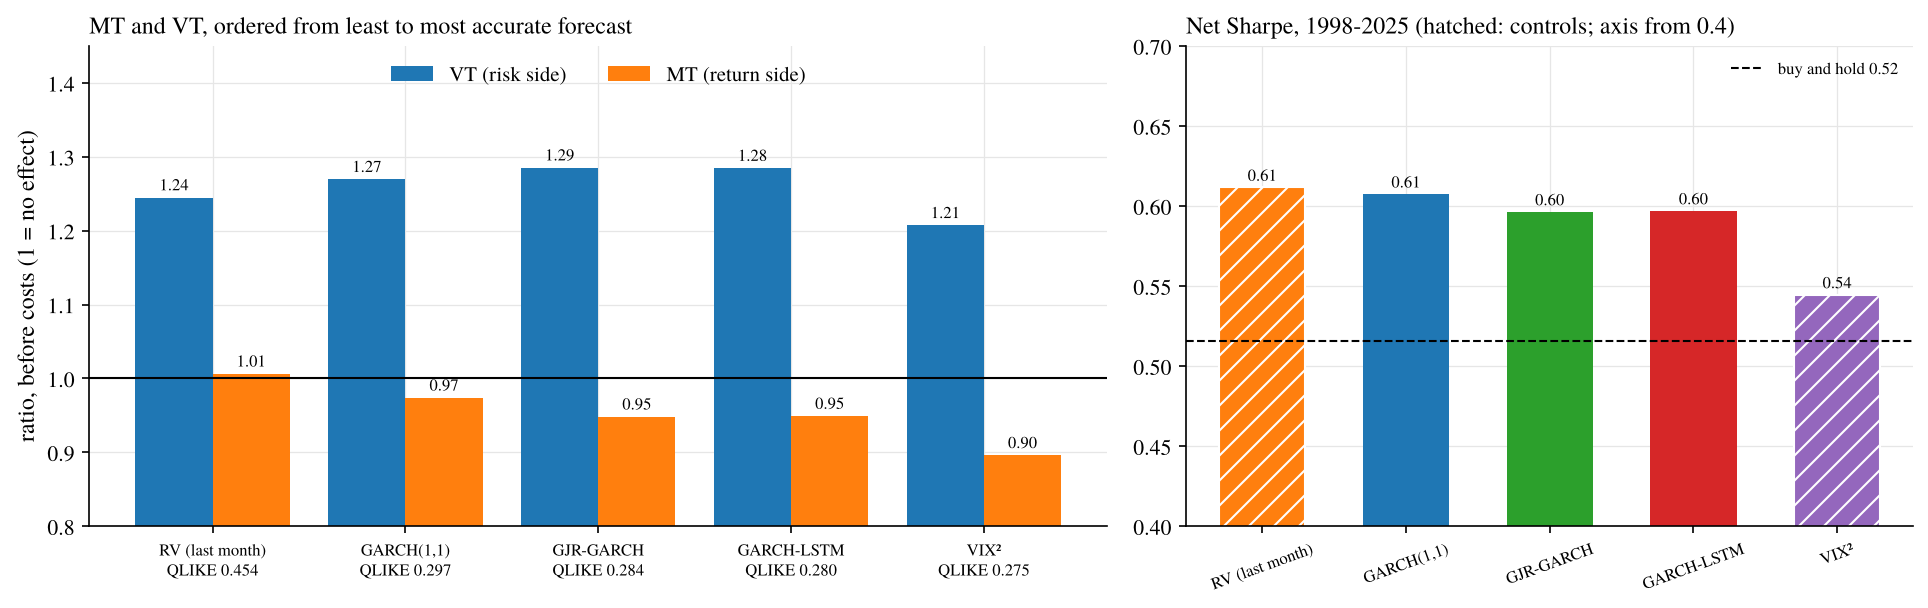
\includegraphics[width=0.95\textwidth]{figs/fig04_mt_vt.png}
\caption{Left: mean timing (MT) and variance timing (VT), from least to most accurate forecast. Right: net Sharpe ratio (hatched: controls).}
\label{fig:mtvt}
\end{figure}

\FloatBarrier
\subsection{Why not? Variance is predictable, returns are not}\label{sec:why}
\paragraph{What can be forecast?} We give returns and variance the same real-time test: an expanding-window predictive regression, re-estimated every month on all available data from 1970, forecasting next month over 1998--2025, with the out-of-sample $R^2$ measured against the historical average (Campbell and Thompson, 2008; Welch and Goyal, 2008) and the one-sided Clark and West (2007) test (Table~\ref{tab:oos}, Figure~\ref{fig:predict}).

\begin{table}[htbp]
\centering\small
\caption{Out-of-sample $R^2$ against the historical average, next month, 1998--2025. The GJR-GARCH and GARCH-LSTM regressions start in 1975, when their forecasts begin.}\label{tab:oos}
\begin{adjustbox}{max width=\linewidth}\begin{tabular}{@{}llcc@{}}
\toprule
Real-time predictor & Target & OOS $R^2$, \% & Clark--West $p$\\
\midrule
GARCH(1,1) forecast & log realised variance & 53.1 & 0.000\\
GJR-GARCH forecast & log realised variance & 53.6 & 0.000\\
GARCH-LSTM forecast & log realised variance & 53.6 & 0.000\\
RV (last month) & log realised variance & 47.1 & 0.000\\
\VIX & log realised variance & 57.1 & 0.000\\
Last month's return & excess return & $-$0.3 & 0.43\\
Past 12 months' return (Moskowitz et al., 2012) & excess return & $-$0.3 & 0.63\\
GARCH(1,1) variance forecast & excess return & $-$2.1 & 0.60\\
Average of the three (Rapach et al., 2010) & excess return & $-$0.6 & 0.57\\
Average, forecast $\ge 0$ (Campbell and Thompson, 2008) & excess return & $-$0.2 & 0.57\\
\bottomrule
\end{tabular}\end{adjustbox}
\end{table}

\begin{figure}[htbp]
\centering
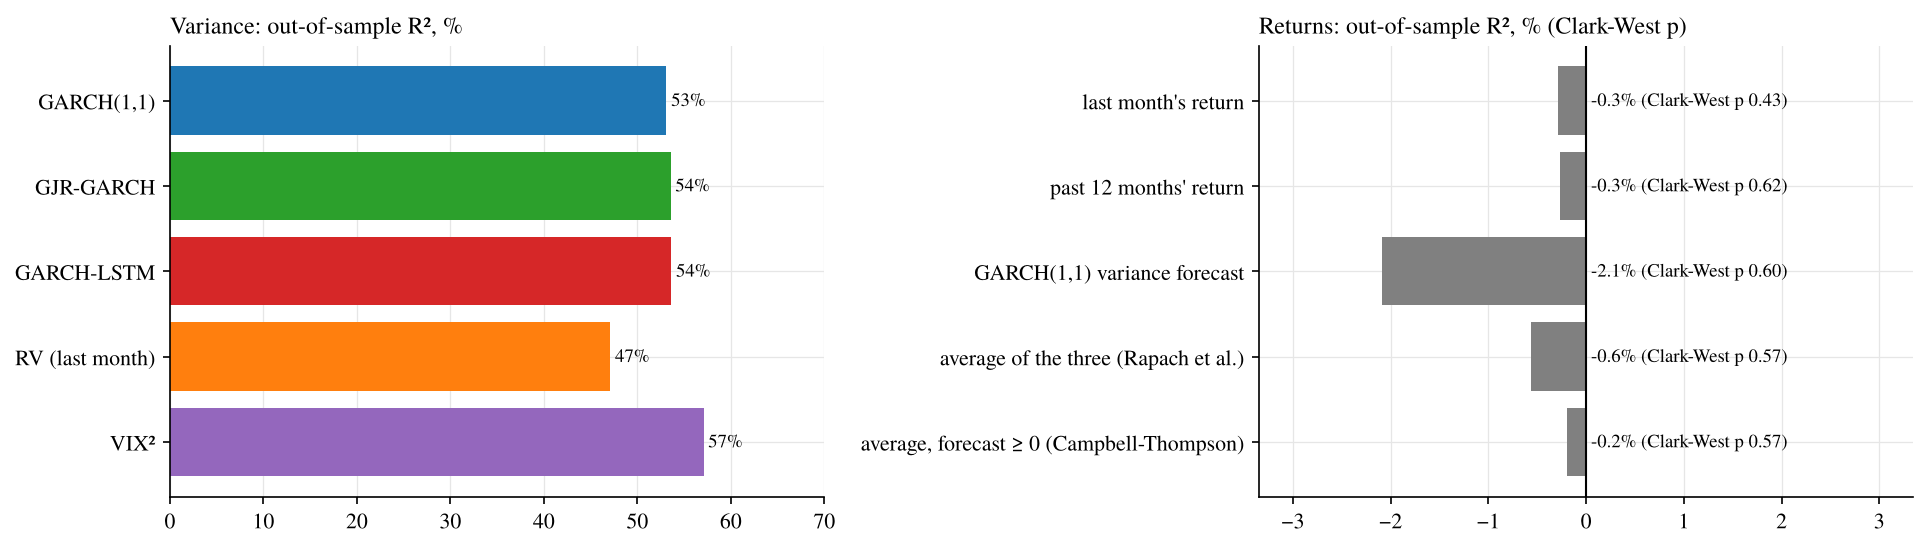
\includegraphics[width=0.95\textwidth]{figs/fig05_predictability.png}
\caption{What can be forecast one month ahead: variance (left) and returns (right); note the different scales.}
\label{fig:predict}
\end{figure}

The variance forecasts explain 47\% to 57\% of next month's log realised variance out of sample; for returns, every predictor does worse than the historical average equity premium. This is why the rule times only variance and treats the expected return as constant, and why a better variance forecast cannot raise MT: the rule has no information to tell the months that pay well from those that do not.

\paragraph{Where the return side leaks: the recovery months.} We split months in real time by last month's volatility: normal (not in its top 20\%, expanding window), panic (top 20\% and still rising, 5-day above 63-day variance) and recovery (top 20\% but already falling), for the Moreira--Muir rule over 1975--2025.

Recovery months have the highest average return (1.6\% a month), but the rule holds the same low exposure in panics and recoveries (0.34 and 0.35): an inverse-variance rule only sees the level of variance, which is high in both states (Table~\ref{tab:states}). A sharper variance forecast, which cuts exposure faster after a spike, makes this worse. The intervals are wide, so this is suggestive, and a simple fix (at least full exposure in recovery months) does not beat plain timing (Sharpe 0.59 against 0.61).

\begin{table}[htbp]
\centering\small
\caption{Market return and timed exposure by volatility state, 1975--2025 (timed on RV).}\label{tab:states}
\begin{adjustbox}{max width=\linewidth}\begin{tabular}{@{}lcccc@{}}
\toprule
State & Months & Market return, \%/month & Naive 95\% interval & Average exposure\\
\midrule
Normal & 434 & 0.64 & $\pm$0.36 & 1.20\\
Panic & 81 & 0.37 & $\pm$1.26 & 0.34\\
Recovery & 97 & 1.59 & $\pm$1.16 & 0.35\\
\bottomrule
\end{tabular}\end{adjustbox}
\end{table}

\FloatBarrier
\subsection{Q3: does training the forecast for the decision help?}\label{sec:q3}

\begin{table}[htbp]
\centering\footnotesize
\caption{Accuracy-trained (Acc) vs decision-trained (Dec) forecasts on six factors, 1998--2025. Every forecast goes through the full rule (cap 1.5, 10 bp, $c$ reset every January); GARCH-LSTM: ensemble of 5 seeds.}\label{tab:q3}
\setlength{\tabcolsep}{3.5pt}
\begin{adjustbox}{max width=\linewidth}\begin{tabular}{@{}lccccccccccccc@{}}
\toprule
 & B\&H & \multicolumn{4}{c}{Net Sharpe ratio} & \multicolumn{4}{c}{Realised objective, \% p.a.} & \multicolumn{4}{c}{QLIKE (diagnostic)}\\
\cmidrule(lr){3-6}\cmidrule(lr){7-10}\cmidrule(lr){11-14}
 & SR & \multicolumn{2}{c}{GJR} & \multicolumn{2}{c}{LSTM} & \multicolumn{2}{c}{GJR} & \multicolumn{2}{c}{LSTM} & \multicolumn{2}{c}{GJR} & \multicolumn{2}{c}{LSTM}\\
Factor & & Acc & Dec & Acc & Dec & Acc & Dec & Acc & Dec & Acc & Dec & Acc & Dec\\
\midrule
Mkt & 0.516 & 0.597 & 0.573 & 0.597 & 0.537 & 3.46 & 3.21 & 3.47 & 2.68 & 0.284 & 0.285 & 0.280 & 0.587\\
SMB & 0.111 & 0.002 & $-$0.063 & 0.006 & $-$0.079 & $-$1.48 & $-$2.04 & $-$1.45 & $-$2.99 & 0.192 & 0.198 & 0.188 & 0.322\\
HML & 0.080 & 0.052 & 0.057 & 0.051 & $-$0.068 & $-$0.93 & $-$0.96 & $-$0.95 & $-$2.07 & 0.338 & 0.445 & 0.339 & 0.449\\
Mom & 0.210 & 0.553 & 0.537 & 0.548 & 0.532 & 2.98 & 2.81 & 2.93 & 2.78 & 0.271 & 0.259 & 0.250 & 0.424\\
RMW & 0.367 & 0.321 & 0.321 & 0.319 & \textbf{0.427} & 1.02 & 1.02 & 1.01 & \textbf{1.79} & 0.193 & 0.226 & 0.194 & 0.709\\
CMA & 0.241 & 0.052 & 0.114 & 0.054 & 0.085 & $-$0.55 & $-$0.36 & $-$0.55 & $-$0.43 & 0.184 & 0.270 & 0.187 & 1.087\\
\bottomrule
\end{tabular}\end{adjustbox}
\end{table}

\begin{itemize}
\item \textbf{On its own objective, Dec loses.} This is the primary yardstick, since it is what Dec was trained to maximise. The decision-trained GARCH-LSTM beats the accuracy-trained network out of sample on only 2 of 6 factors (RMW $+$0.78, CMA $+$0.12\% a year) and is worse on average ($-$0.45\% a year). No difference is significant (bootstrap $p$ 0.12 to 0.81, unadjusted).
\item \textbf{On the Sharpe ratio it also loses.} Dec minus Acc is $-$0.06 on the market, $-$0.09 on SMB, $-$0.12 on HML and $-$0.02 on momentum, against $+$0.11 on RMW and $+$0.03 on CMA (average $-$0.02). After the Romano--Wolf adjustment over the 12 Sharpe comparisons no $p$-value for the GARCH-LSTM is below 0.70.
\item \textbf{The control.} For GJR-GARCH, with few parameters, Dec minus Acc in the Sharpe ratio is between $-$0.06 and $+$0.06 (average $-$0.01), and the realised objective is lower on 5 of 6 factors. Dec is slightly but consistently worse on the market ($-$0.023, bootstrap $p=0.017$) and SMB ($-$0.064, $p=0.025$); neither survives the Romano--Wolf adjustment ($p=0.13$ and $0.11$).
\item \textbf{On the market,} the decision-trained GARCH-LSTM is the weakest timed portfolio (Table~\ref{tab:perf}: Sharpe 0.537, volatility 12.8\%, worst drawdown $-$37.9\%). Its Sharpe gain over buy and hold is $+$0.02 ($p=0.84$; Ledoit--Wolf $p=0.84$), and against the accuracy-trained network $-$0.06 ($p=0.30$).
\item \textbf{The price: worse forecasts.} The decision-trained network's forecasts are 1.3 (HML) to 5.8 (CMA) times worse in QLIKE, and still 1.5 to 4.1 times worse after rescaling each forecast by its best constant, so Dec gives up tracking of volatility, not only calibration.
\item \textbf{The network adds little even when trained for accuracy.} The accuracy-trained GARCH-LSTM and GJR-GARCH have almost the same Sharpe ratio on every factor (within 0.005).
\end{itemize}
\textit{Answer to Q3: no.} Decision-focused learning accepts a worse forecast in exchange for a better decision; here the network pays the price without obtaining the benefit. This tests one design, not decision-focused learning in general.

\begin{figure}[htbp]
\centering
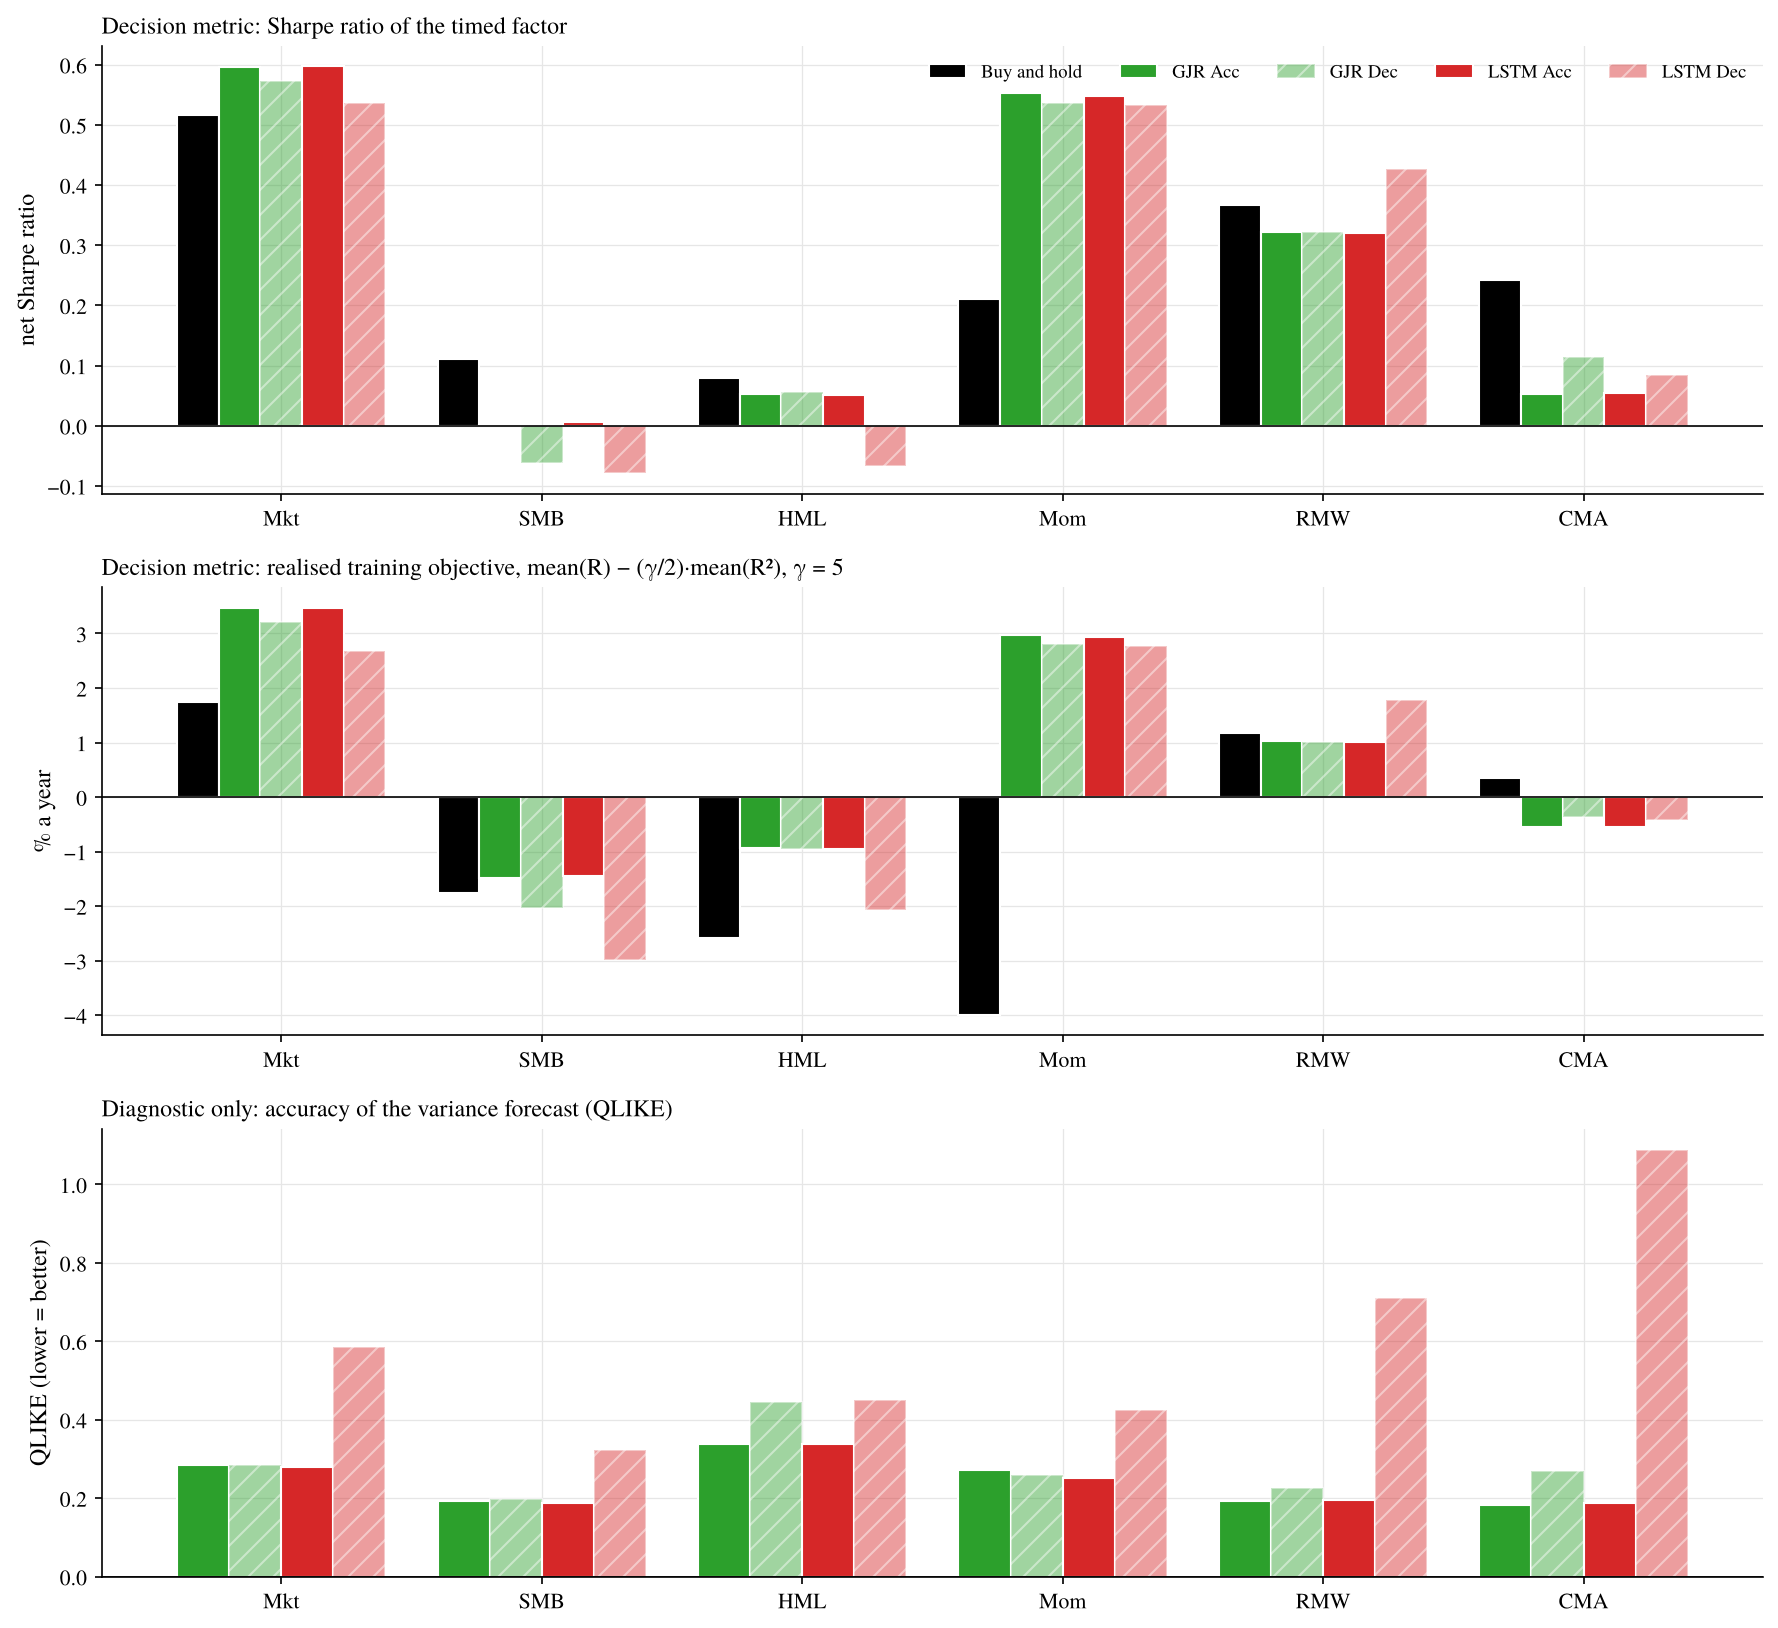
\includegraphics[width=0.9\textwidth]{figs/fig06_acc_vs_dec.png}
\caption{Acc vs Dec: net Sharpe ratio, realised training objective and QLIKE on the six factors, 1998--2025.}
\label{fig:accdec}
\end{figure}

\FloatBarrier
\subsection{Other benchmarks}\label{sec:otherbench}

\begin{table}[htbp]
\centering\small
\caption{Common window of the course CRSP file, February 2000 -- December 2020. Timed portfolios net of costs; passive benchmarks without costs. ``At market vol'': each series rescaled after the fact to the market's volatility.}\label{tab:bench}
\begin{adjustbox}{max width=\linewidth}\begin{tabular}{@{}lcccccc@{}}
\toprule
Portfolio & Sharpe & Sortino & Vol, \% & Max DD, \% & Max DD at market vol, \% & Vol of vol, \%\\
\midrule
Buy and hold (S\&P 500 proxy) & 0.435 & 0.624 & 15.8 & $-$50.3 & $-$50.3 & 6.1\\
EW six factors & \textbf{0.752} & \textbf{1.206} & 4.6 & $-$12.2 & $-$37.4 & 2.1\\
EW CRSP stocks & 0.497 & 0.770 & 22.1 & $-$59.0 & $-$45.7 & 8.8\\
Timed, RV & 0.558 & 0.821 & 10.7 & $-$21.3 & $-$32.6 & 3.1\\
Timed, GARCH(1,1) & 0.560 & 0.825 & 10.8 & $-$25.1 & $-$37.2 & 2.9\\
Timed, GJR-GARCH & 0.562 & 0.829 & 10.8 & $-$26.3 & $-$38.6 & 2.7\\
Timed, GARCH-LSTM & 0.560 & 0.822 & 11.2 & $-$28.7 & $-$40.4 & 2.6\\
\bottomrule
\end{tabular}\end{adjustbox}
\end{table}

Over 2000--2020 the equal-weighted factor mix has by far the best Sharpe ratio (0.75), ahead of the timed market portfolios (0.56), the equal-weighted CRSP stocks (0.50) and the market (0.44). At the market's volatility the timed portfolios lose 33\% to 40\% at worst against 50\% for the market, 46\% for the CRSP stocks and 37\% for the factor mix. Timing beats the market on risk, but diversifying across factors does more for the Sharpe ratio.

%======================================================================
\section{Conclusion}
\begin{enumerate}
\item \textbf{Timing is a risk tool.} Against the S\&P 500 proxy it roughly halves the worst drawdown ($-$50\% to between $-$21\% and $-$29\%; $-$32\% to $-$42\% at equal volatility), lost less in five of six crises, raises the Sortino and Calmar ratios and the certainty equivalent, and makes the portfolio's own risk steadier; only the steadier risk is statistically significant.
\item \textbf{It is not a return engine.} The Sharpe gain is $+$0.08 to $+$0.10, comes from 1998--2015 and is not significant in any period; terminal wealth is lower than buy and hold's because the timed portfolios hold less risk.
\item \textbf{A better forecast does not give a better portfolio.} The accuracy ranking of the five forecasts is close to the reverse of their Sharpe ranking: the least accurate, last month's RV, gives the highest Sharpe ratio and the most accurate, \VIX, the lowest. Mean timing falls from 1.01 to 0.90 as forecasts become more informative, while variance timing stays between 1.21 and 1.29. The GARCH-LSTM is barely more accurate than its GJR base and gives the same Sharpe ratio.

\textit{Why.} Variance is predictable one month ahead, returns are not, so the rule assumes a constant expected return and holds little of the market in the high-return recovery months.
\item \textbf{Training for the decision does not fix it.} With the rule, its cap, its costs and the January reset of $c$ inside the loss, the decision-trained GARCH-LSTM does worse than the accuracy-trained network on its own objective on average and on the Sharpe ratio on 4 of 6 factors, with forecasts 1.3 to 5.8 times worse, and no difference survives the multiple-testing adjustment.
\end{enumerate}
\paragraph{The open question is return information.} The best market rule we found, Xu's switches (Appendix~\ref{app:xu}), works through a 12-month trend filter, a signal about expected returns rather than a better volatility forecast. A decision-focused model would need inputs that carry information about $\mu_t$, not only about $\sigma_t^2$, to improve mean timing.

\paragraph{Limitations.} The data are revised history; VIX before 2003 is back-calculated; drawdowns are month-end; leverage is financed without a spread; equal-volatility figures are diagnostics. The 1998 start, the cap and the rules compared were settled during earlier exploration of the same data, so the multiple-testing adjustments cover the reported comparisons, not that exploration. GJR-GARCH and the GARCH-LSTM keep parameters fitted before a five-year validation block, while GARCH(1,1) is refitted every year. Decision training is one design: one-day forecasts carried 21 days forward, one value of $\gamma$, and an in-sample versus out-of-sample comparison of the objective that we have not run.


\section*{References}
\addcontentsline{toc}{section}{References}
\begingroup\small\setlength{\parindent}{0pt}\raggedright
\hangindent=1.5em\hangafter=1 Andersen, T. G., and Bollerslev, T. (1998). Answering the skeptics: Yes, standard volatility models do provide accurate forecasts. \textit{International Economic Review}, 39(4), 885--905.\par\smallskip
\hangindent=1.5em\hangafter=1 Barroso, P., and Santa-Clara, P. (2015). Momentum has its moments. \textit{Journal of Financial Economics}, 116(1), 111--120.\par\smallskip
\hangindent=1.5em\hangafter=1 Black, F. (1976). Studies of stock price volatility changes. \textit{Proceedings of the 1976 Meetings of the American Statistical Association, Business and Economic Statistics Section}, 177--181.\par\smallskip
\hangindent=1.5em\hangafter=1 Bollerslev, T. (1986). Generalized autoregressive conditional heteroskedasticity. \textit{Journal of Econometrics}, 31(3), 307--327.\par\smallskip
\hangindent=1.5em\hangafter=1 Bollerslev, T., Tauchen, G., and Zhou, H. (2009). Expected stock returns and variance risk premia. \textit{Review of Financial Studies}, 22(11), 4463--4492.\par\smallskip
\hangindent=1.5em\hangafter=1 Bongaerts, D., Kang, X., and van Dijk, M. (2020). Conditional volatility targeting. \textit{Financial Analysts Journal}, 76(4), 54--71.\par\smallskip
\hangindent=1.5em\hangafter=1 Campbell, J. Y., and Thompson, S. B. (2008). Predicting excess stock returns out of sample: Can anything beat the historical average? \textit{Review of Financial Studies}, 21(4), 1509--1531.\par\smallskip
\hangindent=1.5em\hangafter=1 Clark, T. E., and West, K. D. (2007). Approximately normal tests for equal predictive accuracy in nested models. \textit{Journal of Econometrics}, 138(1), 291--311.\par\smallskip
\hangindent=1.5em\hangafter=1 Cederburg, S., O'Doherty, M. S., Wang, F., and Yan, X. S. (2020). On the performance of volatility-managed portfolios. \textit{Journal of Financial Economics}, 138(1), 95--117.\par\smallskip
\hangindent=1.5em\hangafter=1 Chicago Board Options Exchange, CBOE Volatility Index: VIX [VIXCLS], retrieved from FRED, Federal Reserve Bank of St. Louis. \url{https://fred.stlouisfed.org/series/VIXCLS}\par\smallskip
\hangindent=1.5em\hangafter=1 Elmachtoub, A. N., and Grigas, P. (2022). Smart ``predict, then optimize''. \textit{Management Science}, 68(1), 9--26.\par\smallskip
\hangindent=1.5em\hangafter=1 French, K. R. Kenneth R. French Data Library. \url{https://mba.tuck.dartmouth.edu/pages/faculty/ken.french/data_library.html}\par\smallskip
\hangindent=1.5em\hangafter=1 French, K. R., Schwert, G. W., and Stambaugh, R. F. (1987). Expected stock returns and volatility. \textit{Journal of Financial Economics}, 19(1), 3--29.\par\smallskip
\hangindent=1.5em\hangafter=1 Glosten, L. R., Jagannathan, R., and Runkle, D. E. (1993). On the relation between the expected value and the volatility of the nominal excess return on stocks. \textit{Journal of Finance}, 48(5), 1779--1801.\par\smallskip
\hangindent=1.5em\hangafter=1 Harvey, C. R., Hoyle, E., Korgaonkar, R., Rattray, S., Sargaison, M., and Van Hemert, O. (2018). The impact of volatility targeting. \textit{Journal of Portfolio Management}, 45(1), 14--33.\par\smallskip
\hangindent=1.5em\hangafter=1 Künsch, H. R. (1989). The jackknife and the bootstrap for general stationary observations. \textit{Annals of Statistics}, 17(3), 1217--1241.\par\smallskip
\hangindent=1.5em\hangafter=1 Ledoit, O., and Wolf, M. (2008). Robust performance hypothesis testing with the Sharpe ratio. \textit{Journal of Empirical Finance}, 15(5), 850--859.\par\smallskip
\hangindent=1.5em\hangafter=1 Moreira, A., and Muir, T. (2017). Volatility-managed portfolios. \textit{Journal of Finance}, 72(4), 1611--1644.\par\smallskip
\hangindent=1.5em\hangafter=1 Moskowitz, T. J., Ooi, Y. H., and Pedersen, L. H. (2012). Time series momentum. \textit{Journal of Financial Economics}, 104(2), 228--250.\par\smallskip
\hangindent=1.5em\hangafter=1 Newey, W. K., and West, K. D. (1987). A simple, positive semi-definite, heteroskedasticity and autocorrelation consistent covariance matrix. \textit{Econometrica}, 55(3), 703--708.\par\smallskip
\hangindent=1.5em\hangafter=1 Patton, A. J. (2011). Volatility forecast comparison using imperfect volatility proxies. \textit{Journal of Econometrics}, 160(1), 246--256.\par\smallskip
\hangindent=1.5em\hangafter=1 Politis, D. N., and Romano, J. P. (1992). A circular block-resampling procedure for stationary data. In R. LePage and L. Billard (Eds.), \textit{Exploring the Limits of Bootstrap} (pp. 263--270). Wiley.\par\smallskip
\hangindent=1.5em\hangafter=1 Rapach, D. E., Strauss, J. K., and Zhou, G. (2010). Out-of-sample equity premium prediction: Combination forecasts and links to the real economy. \textit{Review of Financial Studies}, 23(2), 821--862.\par\smallskip
\hangindent=1.5em\hangafter=1 Romano, J. P., and Wolf, M. (2005). Stepwise multiple testing as formalized data snooping. \textit{Econometrica}, 73(4), 1237--1282.\par\smallskip
\hangindent=1.5em\hangafter=1 Shumway, T. (1997). The delisting bias in CRSP data. \textit{Journal of Finance}, 52(1), 327--340.\par\smallskip
\hangindent=1.5em\hangafter=1 Welch, I., and Goyal, A. (2008). A comprehensive look at the empirical performance of equity premium prediction. \textit{Review of Financial Studies}, 21(4), 1455--1508.\par\smallskip
\hangindent=1.5em\hangafter=1 Xu, X. (2024). Improving volatility-managed portfolios in real time. Working paper, ESSCA School of Management. SSRN 4778937. \url{https://ssrn.com/abstract=4778937}\par\smallskip
\hangindent=1.5em\hangafter=1 Zhao, P., Zhu, H., Ng, W. S. H., and Lee, D. L. (2024). From GARCH to neural network for volatility forecast. \textit{Proceedings of the AAAI Conference on Artificial Intelligence}, 38(15), 16998--17006.\par\smallskip
\endgroup

\startappendices
%======================================================================
\section{Xu's switches and conditional timing}\label{app:xu}
Xu (2024) starts from the Moreira--Muir rule and adds two switches (his eq.~11),
\[
w_t=C_t\Bigl(\frac{c^*}{RV_{t-1}}\Bigr)^{I_t},
\]
where $c^*$ is a fixed target variance (12\% a year) and $I_t$, $C_t$ are two 0/1 switches set with data up to month $t-1$: an intercept switch ($I_t=0$, so $w_t=1$ and no timing, if the 60-month regression of returns on last month's variance has a non-positive intercept) and a cash switch ($C_t=0$, cash, if the past 12 months' return is negative). Conditional timing (Bongaerts et al., 2020) applies our rule only in the calmest and most volatile 20\% of months.

\begin{table}[htbp]
\centering\small
\caption{Xu's switches on top of our GARCH(1,1) rule, 1998--2025, net of costs.}\label{tab:xu}
\begin{adjustbox}{max width=\linewidth}\begin{tabular}{@{}lccccccc@{}}
\toprule
Rule & SR 98--25 & SR 98--15 & SR 16--25 & Sortino & Max DD eq.\ vol, \% & MT & VT\\
\midrule
Timed, GARCH(1,1) (ours) & 0.608 & 0.460 & 0.828 & 0.909 & $-$36.9 & 0.974 & 1.269\\
+ intercept switch only & 0.589 & 0.435 & 0.833 & 0.875 & $-$47.8 & 0.976 & 1.221\\
+ cash switch only & 0.657 & 0.589 & 0.765 & 1.005 & $-$28.4 & 1.096 & 1.218\\
+ both (Xu switches) & 0.679 & 0.625 & 0.771 & 1.045 & $-$28.7 & 1.141 & 1.203\\
Xu as in his paper & 0.615 & 0.622 & 0.615 & 0.924 & $-$34.4 & 1.100 & 1.147\\
Conditional (Bongaerts et al.) & 0.619 & 0.449 & 0.878 & 0.933 & $-$40.9 & 1.035 & 1.199\\
\bottomrule
\end{tabular}\end{adjustbox}
\end{table}

The cash switch, a time-series momentum filter (Moskowitz et al., 2012), does most of the work: it gains on the return side (MT 1.14), not through better volatility timing. Against buy and hold Xu's switches gain $+$0.16 of Sharpe (bootstrap $p=0.35$), $+$0.28 before 2016 and $-$0.05 after; not significant.

%======================================================================
\section{Building the rule one piece at a time}\label{app:buildup}

\begin{table}[htbp]
\centering\small
\caption{Rule build-up with the GARCH(1,1) forecast, 1998--2025; drawdowns and vol of vol at buy and hold's volatility.}\label{tab:buildup}
\begin{adjustbox}{max width=\linewidth}\begin{tabular}{@{}lcccccc@{}}
\toprule
Step & Sharpe & Sortino & Max DD, \% & Vol of vol, \% & Traded/yr & MT\\
\midrule
1. Buy and hold & 0.516 & 0.748 & $-$50.3 & 5.76 & 0.00 & 1.000\\
2. Scale by $1/\sigma$ (vol target), no cap, no costs & 0.614 & 0.908 & $-$42.8 & 3.51 & 2.36 & 0.986\\
3. Scale by $1/\sigma^2$ instead (Moreira--Muir) & 0.608 & 0.897 & $-$34.1 & 5.17 & 3.89 & 0.953\\
4. + cap exposure at 1.5 & 0.637 & 0.960 & $-$36.4 & 4.20 & 3.28 & 0.974\\
5. + 10 bp trading costs (our rule) & 0.608 & 0.909 & $-$36.9 & 4.19 & 3.28 & 0.974\\
6. $c$ set once (1970--1997) instead of every January & 0.574 & 0.843 & $-$39.3 & 4.17 & 3.24 & 0.932\\
\bottomrule
\end{tabular}\end{adjustbox}
\end{table}

Volatility scaling (Harvey et al., 2018) already lifts the Sharpe ratio to 0.61; variance scaling cuts the drawdown more but lowers MT; the cap helps a little; costs take 0.03; a frozen $c$ loses 0.03 more. Moreira and Muir's full-sample $c$, which looks ahead, gives a lower Sharpe ratio than our real-time $c$ for all five forecasts (by 0.02 to 0.03).

%======================================================================
\section{The six factors and factor exposure over time}\label{app:factors}
Timed on its own GARCH(1,1) forecast, the average Sharpe gain across the six factors is about zero ($+$0.01; 2 of 6 gain), with a smaller drawdown on 4 of 6. Momentum has the largest gain ($+$0.35, Ledoit--Wolf $p=0.02$, Romano--Wolf $p=0.10$), in line with Barroso and Santa-Clara (2015). Figure~\ref{fig:factorexp} shows that the models cut every factor together in crises. The accuracy-trained GJR-GARCH and GARCH-LSTM hold almost the same exposures; only the decision-trained network departs, holding more of the market, SMB and RMW (average SMB exposure 0.83 against 0.77) and less of momentum and CMA.

\begin{figure}[htbp]
\centering
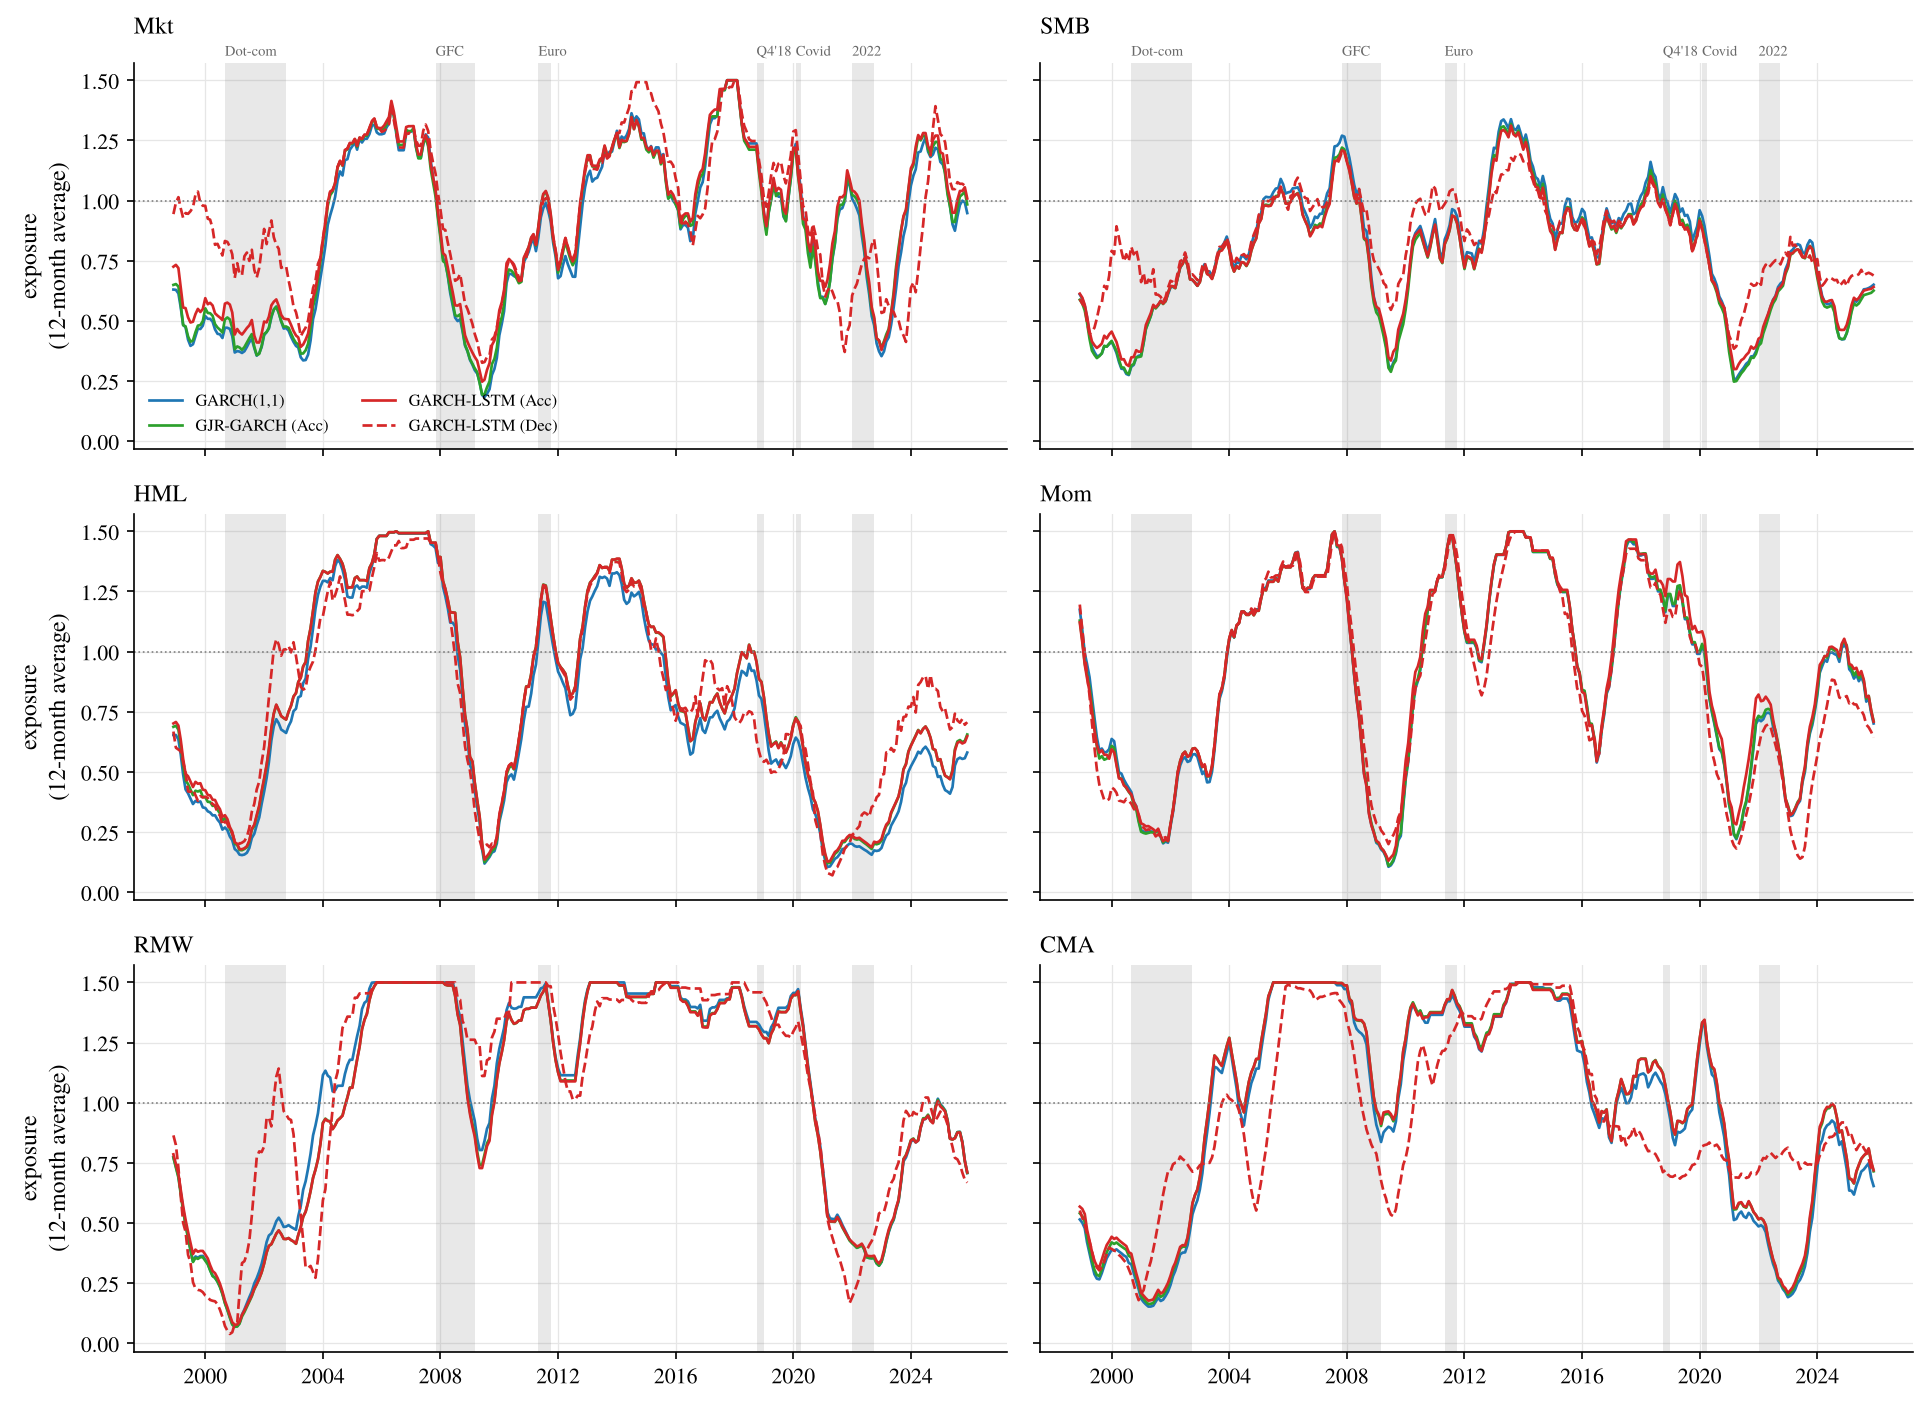
\includegraphics[width=\textwidth]{figs/figC_factor_exposures.png}
\caption{Exposure to each factor (12-month average) under each forecast, 1998--2025. Grey bands: the six crises.}
\label{fig:factorexp}
\end{figure}

%======================================================================
\section{Further checks}\label{app:checks}
\begin{figure}[htbp]
\centering
\begin{subfigure}[t]{0.42\textwidth}\centering
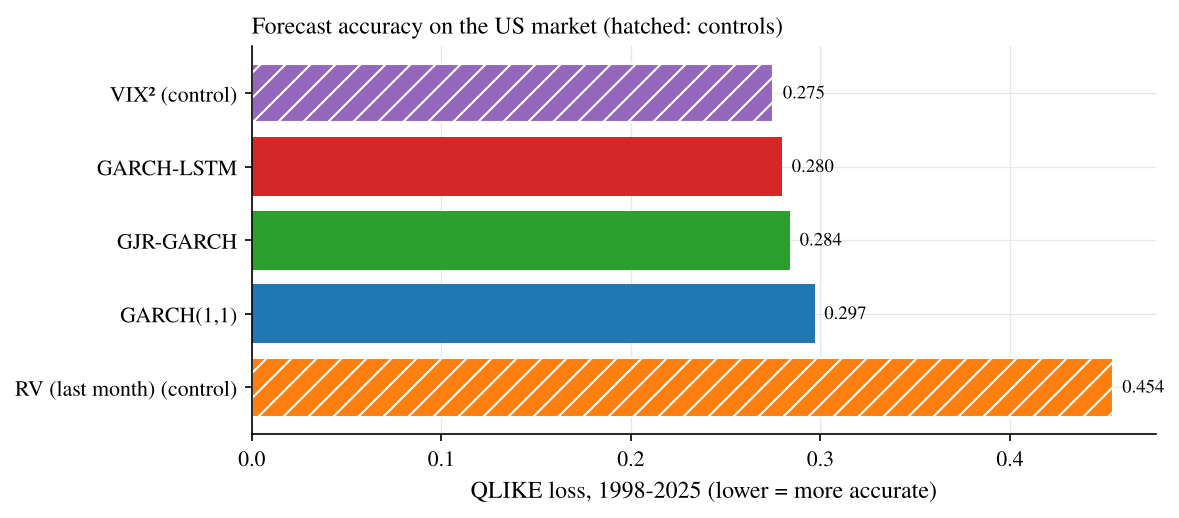
\includegraphics[width=\textwidth]{figs/fig04_qlike.png}
\caption{QLIKE, 1998--2025.}
\end{subfigure}\hfill
\begin{subfigure}[t]{0.55\textwidth}\centering
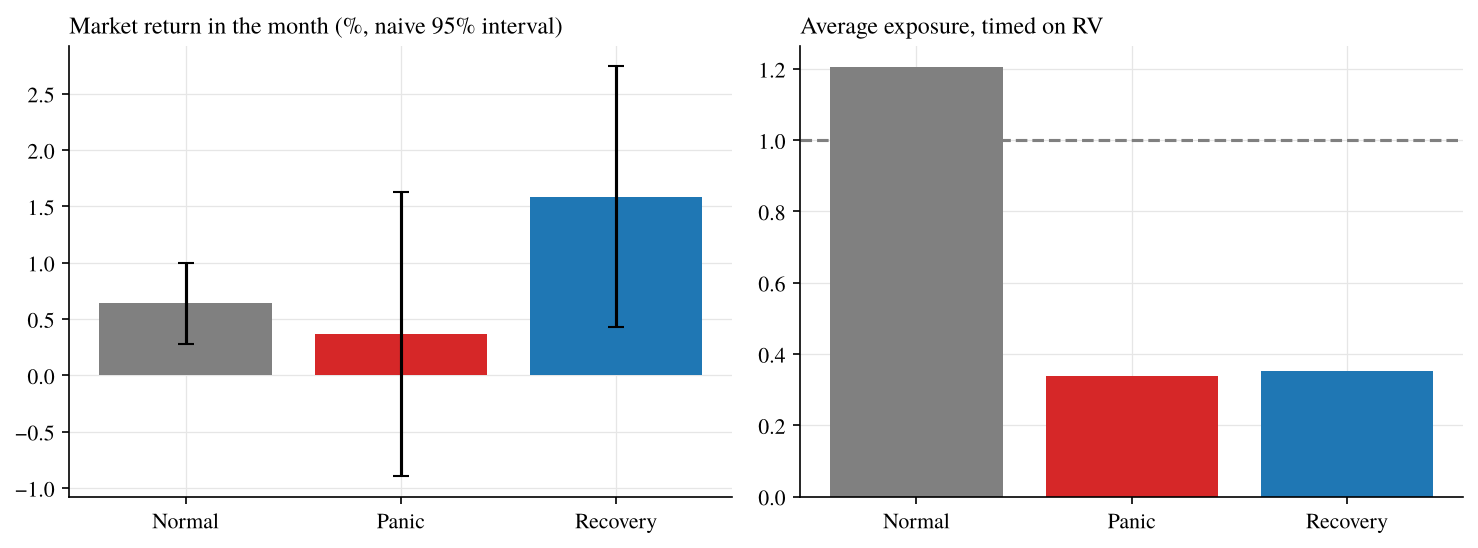
\includegraphics[width=\textwidth]{figs/fig05_recovery.png}
\caption{Recovery months, 1975--2025.}
\end{subfigure}
\caption{Forecast accuracy and the recovery months.}
\label{fig:qlike}
\end{figure}

\begin{figure}[htbp]
\centering
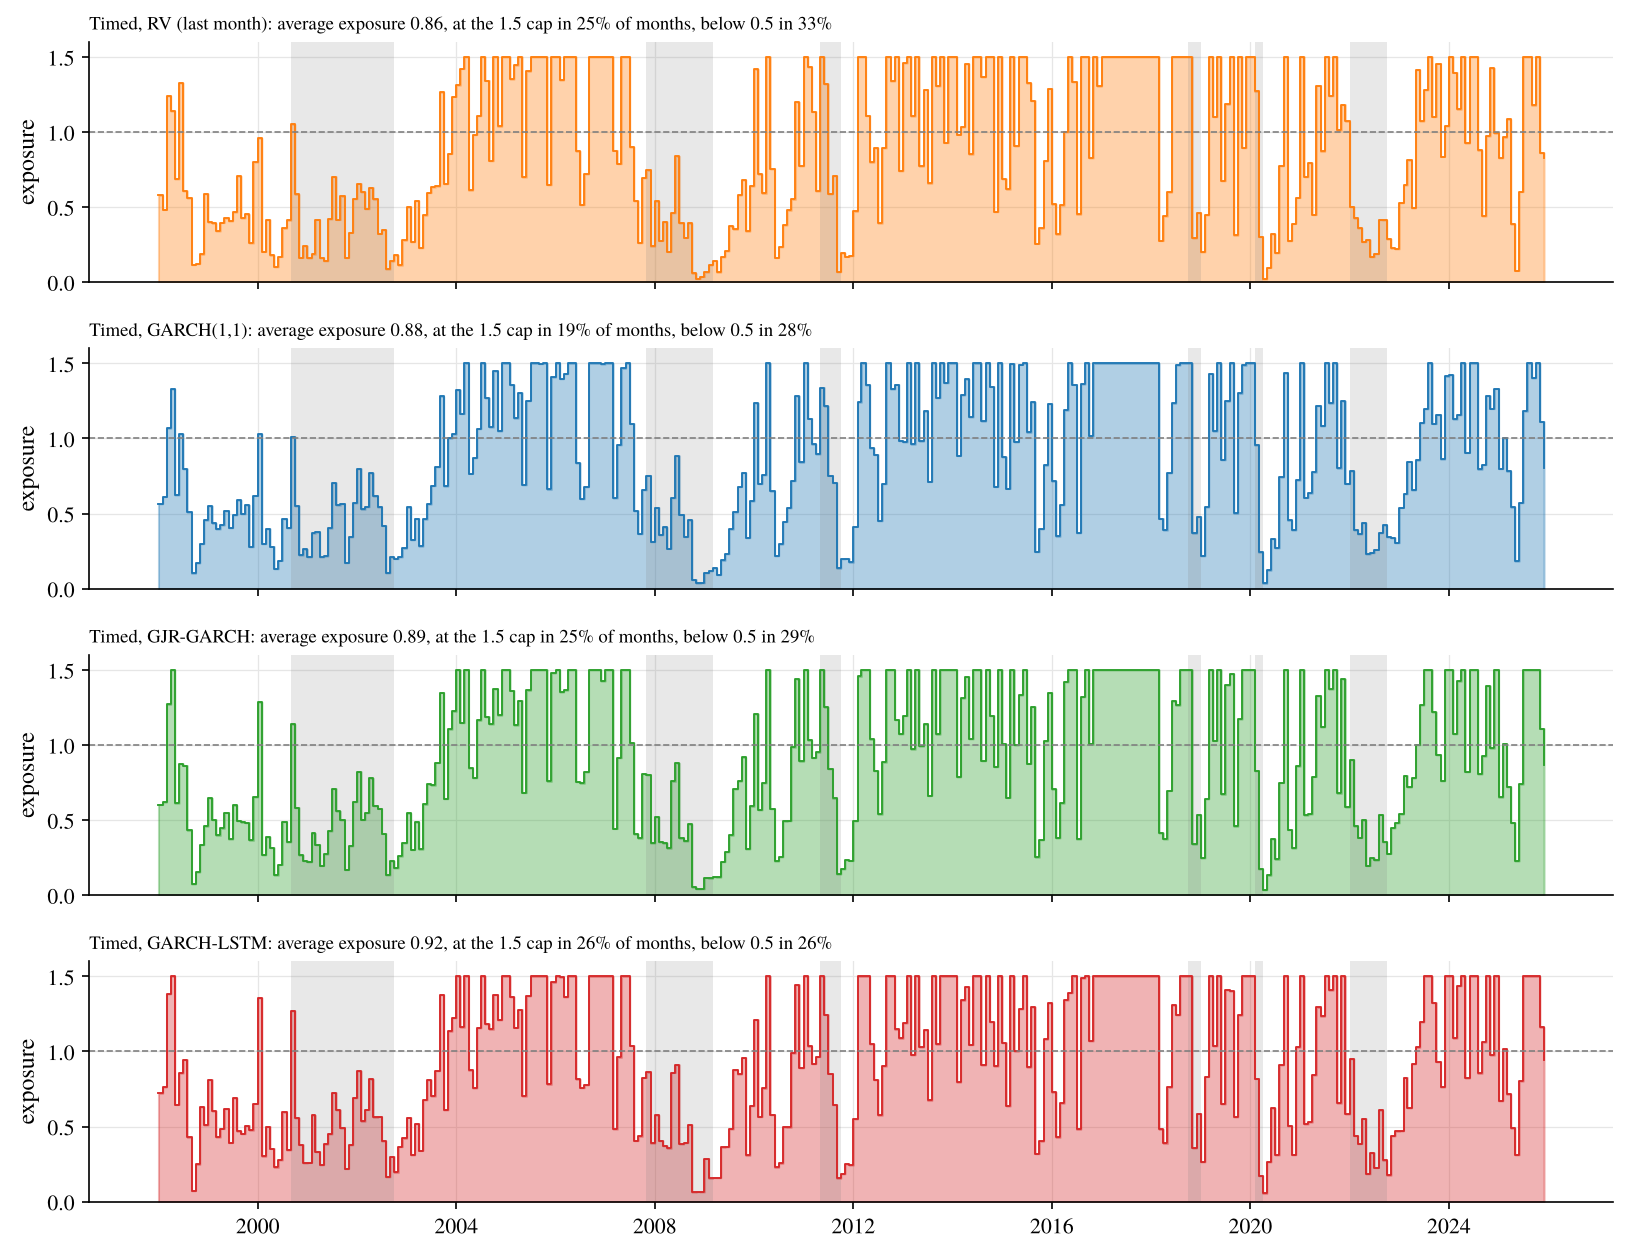
\includegraphics[width=0.72\textwidth]{figs/figE_exposures.png}
\caption{Monthly market exposure chosen by the rule for each timed model, 1998--2025.}
\label{fig:exposures}
\end{figure}

\paragraph{QLIKE by sub-period.} GJR-GARCH and the GARCH-LSTM are the most accurate forecasts in 1998--2015 (both 0.235), \VIX{} in 2016--2025 (0.314, against 0.360 for the GARCH-LSTM) and the GARCH-LSTM in 2021--2025 (0.178); RV is the least accurate everywhere. The Ledoit--Wolf $p$-values of the main comparisons barely move with 0 to 12 HAC lags (e.g.\ GARCH(1,1) vs buy and hold: 0.44 to 0.48).

\paragraph{Reproducibility.} All results come from \texttt{vol\_timing\_final\_revised.ipynb}. The GJR-GARCH and GARCH-LSTM forecasts, scales and exposures come from the full run of \texttt{lstm\_training\_revised.ipynb} (six factors, five seeds, test years 1975--2025), saved in \texttt{data/LSTM-Forecasts-revised/}. The figures in this report were regenerated by running the notebook; the portfolio value curves, calendar-year returns, rolling Sharpe ratios and the extended performance table (CAGR, Calmar ratio, CAPM alpha and beta) are computed from the notebook's own backtest series by \texttt{report\_extras.py}, and the robustness checks quoted in the separate responses to questions by \texttt{qa\_checks.py}. The licensed course CRSP file is not redistributed; without it, only the CRSP benchmark is skipped.

\end{document}
